%-----------------------------------------------------------------
% Link do repozitorijuma na pltaformi GitHub: https://github.com/PosteruOle/master_thesis
%-----------------------------------------------------------------
% Format teze zasnovan je na paketu memoir
% http://tug.ctan.org/macros/latex/contrib/memoir/memman.pdf ili
% http://texdoc.net/texmf-dist/doc/latex/memoir/memman.pdf
% 
% Prilikom zadavanja klase memoir, navedenim opcijama se podešava 
% veličina slova (12pt) i jednostrano štampanje (oneside).
% Ove parametre možete menjati samo ako pravite nezvanične verzije
% mastera za privatnu upotrebu (na primer, u b5 varijanti ima smisla 
% smanjiti 
\documentclass[12pt,oneside]{memoir}

% Paket koji definiše sve specifičnosti mastera Matematičkog fakulteta
\usepackage[latinica]{matfmaster}
%
% Podrazumevano pismo je ćirilica.
%   Ako koristite pdflatex, a ne xetex, sav latinički tekst na srpskom jeziku
%   treba biti okružen sa \lat{...} ili \begin{latinica}...\end{latinica}.
%
% Opicija [latinica]:
%   ako želite da pišete latiniciom, dodajte opciju "latinica" tj.
%   prethodni paket uključite pomoću: \usepackage[latinica]{matfmaster}.
%   Ako koristite pdflatex, a ne xetex, sav ćirilički tekst treba biti
%   okružen sa \cir{...} ili \begin{cirilica}...\end{cirilica}.
%
% Opcija [biblatex]:
%   ako želite da koristite reference na više jezika i umesto paketa
%   bibtex da koristite BibLaTeX/Biber, dodajte opciju "biblatex" tj.
%   prethodni paket uključite pomoću: \usepackage[biblatex]{matfmaster}
%
% Opcija [b5paper]:
%   ako želite da napravite verziju teze u manjem (b5) formatu, navedite
%   opciju "b5paper", tj. prethodni paket uključite pomoću: 
%   \usepackage[b5paper]{matfmaster}. Tada ima smisla razmisliti o promeni
%   veličine slova (izmenom opcije 12pt na 11pt u \documentclass{memoir}).
%
% Naravno, opcije je moguće kombinovati.
% Npr. \usepackage[b5paper,biblatex]{matfmaster}

% Pomoćni paket koji generiše nasumičan tekst u kojem se javljaju sva slova
% azbuke (nema potrebe koristiti ovo u pravim disertacijama)
\usepackage{pangrami}
\usepackage{graphicx}
\usepackage{minted}
\usepackage{tikz}
\usetikzlibrary{shapes.geometric, arrows}
\usetikzlibrary{positioning}
\graphicspath{ {./assets/} }
\tikzstyle{ellibig}=[draw, ellipse, fill=white!50, 
					draw=black!50, top color=white, bottom color=black!10,
					minimum height=8mm, text width=6em, text centered]
\tikzstyle{ellismall}=[draw, ellipse, fill=white!50, 
					draw=black!50, top color=white, bottom color=black!10,
					minimum height=3mm, text width=1.5cm, text centered]     


% Paket koji obezbeđuje ispravni prikaz ćiriličkih italik slova kada
% se koristi pdflatex. Zakomentarisati ako na sistemu koji koristite ovaj
% paket nije dostupan ili ako ne radi ispravno.
\usepackage{cmsrb}
\usepackage{hyperref}
% Ostali paketi koji se koriste u dokumentu
\usepackage{listings} % listing programskog koda

\usepackage{pgfplots}
\pgfplotsset{width=13cm,compat=1.9}
% Datoteka sa literaturom u BibTex tj. BibLaTeX/Biber formatu
\bib{PetarTesicMasterRad}

% Ime kandidata na srpskom jeziku (u odabranom pismu)
\autor{Petar Tešić}
% Naslov teze na srpskom jeziku (u odabranom pismu)
\naslov{Automatska detekcija i optimizacija algoritma CRC u okviru kompajlerske infrastrukture LLVM}
% Godina u kojoj je teza predana komisiji
\godina{2024}
% Ime i afilijacija mentora (u odabranom pismu)
\mentor{dr Milena Vujošević Janičić, vanredni profesor\\ Univerzitet u Beogradu, Matematički fakultet}
% Ime i afilijacija prvog člana komisije (u odabranom pismu)
\komisijaA{dr Filip Marić, redovni profesor\\ Univerzitet u Beogradu, Matematički fakultet}
% Ime i afilijacija drugog člana komisije (u odabranom pismu)
\komisijaB{dr Mirko Spasić, docent\\ Univerzitet u Beogradu, Matematički fakultet}
% Ime i afilijacija trećeg člana komisije (opciono)
% \komisijaC{}
% Ime i afilijacija četvrtog člana komisije (opciono)
% \komisijaD{}
% Datum odbrane (obrisati ili iskomentarisati narednu liniju ako datum odbrane nije poznat)
\datumodbrane{Septembar, 2024.}

% Apstrakt na srpskom jeziku (u odabranom pismu)
\apstr{
U savremenoj industriji razvoja softvera, efikasnost i optimizacija koda predstavljaju ključne 
aspekte u postizanju visokih performansi računarskih sistema. Ovaj master rad 
istražuje inovativan pristup prevođenju algoritma CRC (eng. \textit{Cyclic Redundancy 
Check}) korišćenjem kompilatorske infrastrukture LLVM. Algoritam CRC detektuje potencijalne 
promene u podacima nastalim usled transfera kroz različite medijume (žičane mreže, bežične 
mreže ili optičke kablove) i ima široku primenu u digitalnoj komunikaciji, gde se koristi za 
proveru integriteta podataka. Zbog svoje učestale primene važno je koristiti optimizovane 
verzije ovog algoritma.
 
Cilj ovog rada je unapređenje infrastrukture LLVM u kontekstu prevođenja algoritma CRC, i na 
taj način ostvarivanje boljih performansi programa koji koriste algoritam CRC i LLVM kao svoj 
kompilator. Osnovna ideja rešenja predstavljenog u radu zasniva se na  
detekciji neoptimizovane verzije algoritma CRC na nivou LLVM međureprezentacije i zamenjivanju funkcionalno ekvivalentnom optimizovanom verzijom. Unapređenje je vidljivo
na različitim procesorskim arhitekturama, specijalno i na procesorskoj arhitekturi RISC-V. 
Rezultati dobijeni testiranjem predstavljenog rešenja pokazuju značajno poboljšanje 
performansi algoritma CRC prevedenog LLVM kompilatorom.
\\
}

% Ključne reči na srpskom jeziku (u odabranom pismu)
\kljucnereci{kompilatorska infrastruktura LLVM, algoritam CRC, arhitektura RISC-V, LLVM 
međureprezentacija, LLVM mašinski zavisan međukod, domenski specifičan jezik TableGen, LLVM 
optimizacioni prolaz}

\begin{document}
% ==============================================================================
% Uvodni deo teze
\frontmatter
% ==============================================================================
% Naslovna strana
\naslovna
% Strana sa podacima o mentoru i članovima komisije
\komisija
% Strana sa posvetom (u odabranom pismu)
\posveta{Zahvaljujem se svojoj porodici, prijateljima, Kaći, profesorki Mileni i svim kolegama iz kompanije SYRMIA na nesebičnoj pomoći i podršci}
% Strana sa podacima o disertaciji na srpskom jeziku
\apstrakt
% Sadržaj teze
\tableofcontents*

% ==============================================================================
% Glavni deo teze
\mainmatter
% ==============================================================================

% ------------------------------------------------------------------------------
\chapter{Uvod}
\label{chap:uvod}
% ------------------------------------------------------------------------------

Programski prevodioci prevode programe iz viših programskih jezika u mašinski k\^od i time omogućavaju izvršavanje softvera na različitim arhitekturama računara. Zahvaljujući optimizacijama koje vrše prevodioci dobija se kvalitetniji izvršivi k\^od, odnosno k\^od koji se izvršava brže, koji zauzima manju količinu memorije ili koji ima bolju energetsku efikasnost. 

Veliki broj softverskih kompanija ulaže značajna finansijska sredstva u razvoj programskih prevodilaca, odnosno u razvoj kompilatorskih infrastruktura, sa ciljem da softver koji oni proizvode ima kvalitetan izvršivi k\^od.
Na primer, kompanije \textit{Apple} \cite{apple}, \textit{Google} \cite{google}, \textit{Nvidia} \cite{nvidia} ulažu u razvoj kompilatorske infrastrukture LLVM \cite{llvm}, kojoj je ovaj rad posvećen. 

LLVM je jedan od najpopularnijih prevodilaca za programske jezike kao što su  \textit{C}, \textit{C++}, \textit{Rust} и \textit{Swift}.
U ovom radu biće predstavljene optimizacije implementirane u okviru kompilatora LLVM koje treba da omoguće efikasniji rezultat prevođenja algoritma CRC \cite{what_is_crc}. Optimizacije su sprovedene na nivou LLVM međureprezentacije. Jedna od optimizacija ima za cilj upotrebu na RISC-V arhitekturi \cite{what_is_riscv}, dok je drugu moguće koristiti i na drugim arhitekturama.

Rad se sastoji od šest poglavlja. U poglavlju \ref{chap:llvm} se govori o procesu prevođenja programa, metodologijama konstrukcije kompilatora i o kompilatorskoj infrastrukturi LLVM. Predstavljena je istorija samog projekta, arhitektura projekta, delovi kompilatora i međureprezentacija koju LLVM koristi. Dodatno, opisana je i infrastruktura za testiranje. 
Poglavlje \ref{chap:crc} je posvećeno algoritmu CRC i problemu njegovog prepoznavanja. Predstavljen je koncept detektovanja grešaka u podacima, zajedno sa trenutnim načinima korekcije i detekcije grešaka. Poglavlje \ref{chap:riscv} je posvećeno procesorskim arhitekturama, sa akcentom na procesorsku arhitekturu RISC-V jer je baš za nju predložena jedna optimizacija u okviru ovog rada. 
U poglavlju \ref{chap:implementacija} su predstavljena dva rešenja problema detektovanja algoritma CRC i njegovog optimizovanja. Na početku poglavlja su opisani ideja i postupak zajednički za oba rešenja, a u nastavku su redom nalaze detalji implementacije svakog od predloženih rešenja.
Poslednja sekcija u poglavlju \ref{chap:implementacija} opisuje rezultate eksperimentalne evaluacije predloženih rešenja. Rezultati pokazuju za čak 35\% bolju vremensku efikasnost programa nad kojim je pokrenuta jedna od predloženih implementacija. U poglavlju \ref{chap:zakljucak} je sumirano sve što je predstavljeno u radu i ostavljene su smernice i sugestije čitaocima rada za dalje istraživanje na temu unapređenja LLVM i drugih kompilatora, a i na temu kompilatorskih optimizacija. 

% ------------------------------------------------------------------------------
\chapter{Kompilatori i projekat LLVM}
\label{chap:llvm}
% ------------------------------------------------------------------------------
 
Izvršavanje programa omogućavaju programski prevodioci koji prevode program iz višeg programskog jezika u k\^od koji računar može da izvrši. Za samo izvršavanje programa, posebno je važna efikasnost koja u velikoj meri zavisi od optimizacija koje programski prevodioci sprovode u toku prevođenja programa.  

\section{Osnovne vrste prevodilaca}
Programski prevodioci mogu vršti kompilaciju programa ili njegovu interpretaciju. Za kompilaciju programa koriste se kompilatori, a za interpretaciju interpreteri.

Kompilatori iliti kompajleri predstavljaju veoma kompleksan softver sposoban da proizvoljan k\^od napisan u nekom višem programskom jeziku konvertuje u kvalitetan mašinski k\^od koji će se potom izvršavati na računaru. Proces kompilacije podrazumeva razdvojenost procesa prevođenja i procesa izvršavanja programa. Kompilacijom se kreira izvršiva datoteka koju je potom moguće pokretati, to jest, izvršavati na računaru proizvoljan broj puta. Za svaku promenu u izvornom kodu potrebno je ponoviti proces kompilacije. Neki od najpoznatijih kompilatora otvorenog koda danas su GCC \cite{gcc}, LLVM, RUSTC \cite{rustc} i GraalVM \cite{graalvm}. Primeri programskih jezika za čije prevođenje je potrebno koristiti kompilaciju su C, C++, Rust i Go. Skica procesa kompilacije prikazana je na slici \ref{tikz:kompilacija}.

\begin{figure}
\centering

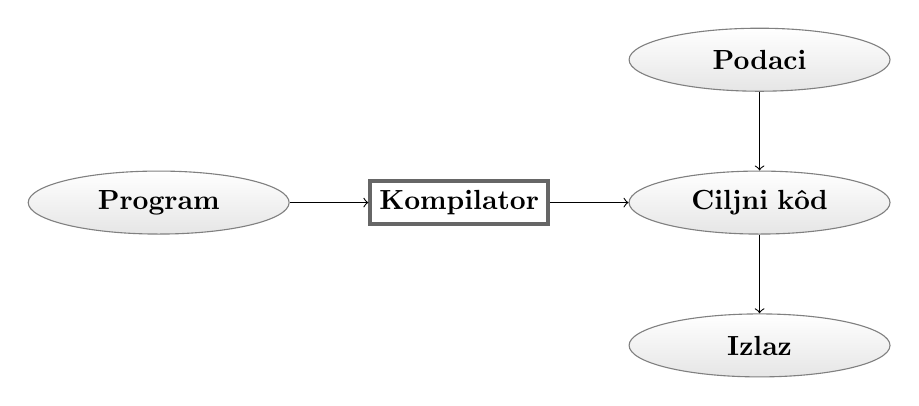
\begin{tikzpicture}[
roundnode/.style={circle, draw=black!60, fill=white!5, very thick, minimum size=7mm},
squarednode/.style={rectangle, draw=black!60, fill=white!5, very thick, minimum size=5mm},
][!ht]

%Nodes
\node[squarednode]      (prevodilac_node)  {\textbf{Kompilator}};
\node[ellibig]        (cilj_node)       [right=of prevodilac_node] {\textbf{Ciljni k\^od}};
\node[ellibig]        (podaci_node)       [above=of cilj_node] {\textbf{Podaci}};
\node[ellibig]        (izlaz_node)       [below=of cilj_node] {\textbf{Izlaz}};

\node[ellibig]        (program_node)       [left=of prevodilac_node] {\textbf{Program}};

%Lines
\draw[->] (program_node.east) -- (prevodilac_node.west);
\draw[->] (prevodilac_node.east) -- (cilj_node.west);
\draw[->] (podaci_node.south) -- (cilj_node.north);
\draw[->] (cilj_node.south) -- (izlaz_node.north);
 
\end{tikzpicture}
\caption{Proces kompilacije i izvršavanja}
\label{tikz:kompilacija}
\end{figure}


Prilikom procesa interpretacije faze prevođenja i izvršavanja programa su 
isprepletane. To znači da se interpretacijom svaka naredba prvo prevodi, a potom se izvršava. 
%Pod prevođenjem naredbe podrazumevamo proveru njene leksičke, sintaksne i semantičke ispravnosti. 
Bilo koja greška u programu biće otkrivena tek kada se prevođenjem i izvršavanjem dođe do linije u kojoj se ona nalazi. Skica procesa interpretacije prikazana je na slici \ref{tikz:interpretacija}. U nastavku rada svako spominjanje procesa prevođenja odnosiće se isključivo na kompilaciju.

\begin{figure}
\centering
 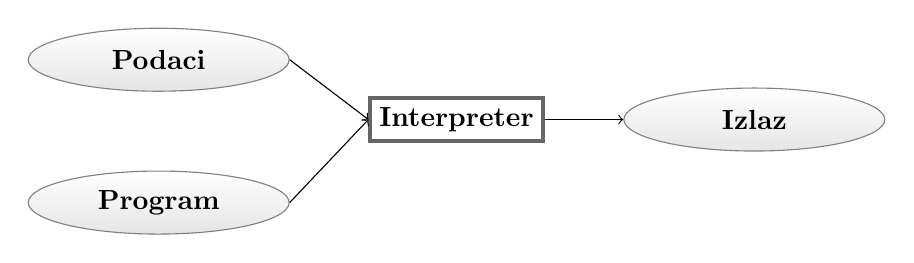
\begin{tikzpicture}[
 roundnode/.style={circle, draw=black!60, fill=white!5, very thick, minimum size=7mm},
 blindnode/.style={circle, draw=white!20, fill=white!5, very thick, minimum size=2mm},
 squarednode/.style={rectangle, draw=black!60, fill=white!5, very thick, minimum size=5mm},
 ][!ht]
 \centering
 %Nodes
 \node[squarednode]      (interpreter_node)  {\textbf{Interpreter}};
 \node[ellibig]        (izlaz_node)       [right=of interpreter_node] {\textbf{Izlaz}};
 \node[ellibig]        (program_node)       [left=of interpreter_node, yshift=-30pt] {\textbf{Program}};
 \node[ellibig]        (podaci_node)       [above=of program_node] {\textbf{Podaci}};

 %Lines
 \draw[->] (program_node.east) -- (interpreter_node.west);
 \draw[->] (interpreter_node.east) -- (izlaz_node.west);
 \draw[->] (podaci_node.east) -- (interpreter_node.west);
 \end{tikzpicture}

\caption{Proces interpretacije i izvršavanja}
\label{tikz:interpretacija}
\end{figure}


\section{Faze prevođenja programa}

U okviru procesa prevođenja programa postoje više različitih faza \cite{dragon_book}: 
\begin{itemize}
 \item leksička analiza, 
\item sintaksička analiza, 
\item semantička analiza,
\item generisanje međukoda,
\item optimizacija međukoda i 
\item generisanje i optimizacija mašinskog koda. 
\end{itemize}
Bitan korak koji se izvršava pre faze leksičke analize, ali koji ne smatramo posebnom fazom prevođenja, jeste pretprocesiranje. U okviru pretprocesiranja se obrađuju direktive poput \texttt{\#include} i \texttt{\#define} direktiva u programskom jeziku \texttt{C}. Korak koji se izvršava nakon prevođenja, a koji takođe ne smatramo posebnom fazom prevođenja, jeste linkovanje. Linkovanjem se kreira jedinstvena izvšiva datoteka od jednog ili više objektnih modula. Objektni moduli mogu nastati ili kompilacijom izvornog koda ili sadržati mašinski k\^od i podatke standardne ili neke nestandardne biblioteke.

U fazi leksičke analize, za koju je odgovaran deo programskog prevodioca koji zovemo leksički 
analizator ili lekser, ustanovljava se da li su u izvornom kodu iskorišćene samo dopustive 
lekseme iliti tokeni. Pod dopustivim leksemama podrazumevamo reči napisane u izvornom kodu 
koje mogu biti prepoznate konačnim automatima kreiranim na osnovu odgovarajućih regularnih 
izraza. Regularni izrazi imaju za cilj da opišu imena promenljivih, ključne reči, operatore, 
separatore i tako dalje. 

Ukoliko je program koji prevodimo sačinjen isključivo od dopustivih 
leksema, u tom slučaju niz prepoznatih leksema se prosleđuje delu programskog prevodioca 
zaduženom za sintaksičku analizu, sintaksičkom analizatoru iliti parseru. U protivnom, u 
slučaju detektovanja nedopustive lekseme, proces prevođenja se zaustavlja i programski 
prevodilac nam saopštava poruku o leksičkoj greški. 

U narednoj fazi, fazi sintaksičke analize, proverava se da li su prepoznate lekseme složene u 
skladu sa gramatikom programskog jezika u kome je izvorni k\^od napisan. 
Pravila slaganja leksema odnosno formiranja rečeničnih konstrukcija se zadaju korišćenjem 
kontekstno-slobodne gramatike (eng. \textit{context-free grammar}). 

Prolaskom kroz naredbe programa i korišćenjem potisnih automata (kreiranim na osnovu gramatike) proverava se da li su instrukcije u skladu sa gramatikom programskog jezika. Ukoliko jesu, na osnovu njih se gradi stablo parsiranja (eng. \textit{parse tree}). 

%Promenjeno!!!!!!
Stablo parsiranja je struktura nalik stablu koja predstavlja sintaksičku strukturu programa. Sastoji se od čvorova, od kojih svaki odgovara elementu programskog jezika u kome je program napisan. Unutrašnji čvorovi stabla parsiranja su predstavljeni neterminalima (ključnim rečima, operatorima, ...), dok su listovi stabla parsiranja predstavljeni terminalima (konstantama, imenima promenljivih, ...). Stablom parsiranja se ne apstrahuju detalji sintakse programskog jezika. Time ova struktura predstavlja detaljniji prikaz izvornog koda i često je korisna za debagovanje. 

Prolaskom kroz stablo parsiranja se prikupljaju informacije o funkcijama, promenljivama i drugim objektima i smeštaju se u tabelu simbola. Korišćenjem tabele simbola proverava se struktura stabla parsiranja. Na osnovu stabla parsiranja se potom kreira apstraktno sintaksno stablo programa (eng. \textit{Abstract Syntax Tree - AST}) \cite{ast}. 

Apstraktno sintaksno stablo je u suštini pojednostavljena verzija stabla parsiranja. 
Čvorovi apstraktnog sintaksnog stabla su apstrahovani od detalja sintakse programskog jezika, što ovu strukturu čini sažetijom i lakšom za čitanje od stabla parsiranja.
Apstraktnim sintaksnim stablom je, takođe, olakšano i zaključivanje o strukturi koda.

U slučaju upotrebe nedozvoljene rečenične konstrukcije, proces prevođenja se zaustavlja i prevodilac nam saopštava poruku o sintaksnoj greški. Ukoliko do takve greške nije došlo, započinje se faza semantičke analize u kojoj se proverava značenje ispravnim rečeničnim konstrukcijama. Provera semantičke ispravnosti programa podrazumeva više nezavisnih provera poput provere tipova, provere labela, provere kontrole toka programa. Na primer, proverom tipova se proverava da li svaka operacija u programu podržana sistemom tipova jezika u kome je program napisan.

Tokom faze generisanja međukoda se od izvornog koda generiše k\^od nezavisan od programskog jezika koji nazivamo međukodom iliti međureprezentacijom. Međureprezentacija služi kao most između visokog nivoa apstrakcije izvornog koda i niskog nivoa apstrakcije instrukcija ciljne arhitekture. Nakon generisanja međukoda sledi faza njegove optimizacije. Faza generisanja mašinskog koda i njegova optimizacija je poslednja faza prevođenja u kojoj se od optimizovanog međukoda dobija krajnji mašinski k\^od za ciljnu procesorsku arhitekturu. Rešenja opisana u ovom radu predstavljaju optimizacije koje se odvijaju upravo u fazama optimizacije međukoda i optimizacije mašinskog koda.

% Cilj ove faze jeste analiziranje i optimizovanje međukoda kako bi se od njega dobio kvalitetan mašinski kod. 

%  Generisani mašinski k\^od se potom optimizuje kako bi mu se smanjio broj instrukcija ili kako bi se određene instrukcije zamenile ekvivalentim, ali efikasnijim instrukcijama. 

% ------------------------------------------------------------------------------
\section{Bitni delovi kompilatora}
\label{sec:kompilatori}
% ------------------------------------------------------------------------------
U arhitekturi većine današnjih kompilatora moguće je uočiti tri bitna dela. 
U pitanju su prednji deo \cite{frontend_quote}, srednji deo \cite{middleend_quote} i zadnji deo \cite{backend_quote} kompilatora.

%Prednji deo kompilatora...
Prednji deo kompilatora (eng. \textit{front end}) je zavisan od višeg programskog jezika kojeg prevodi. Odgovornost prednjeg dela kompilatora jeste obavljanje leksičke, sintaksičke i semantičke analize. Kao rezultat rada prednjeg dela kompilatora generiše se međukod odnosno međureprezentacija (eng. \textit{intermediate representation}) izvornog koda koja se prosleđuje srednjem delu kompilatora.

%Srednji deo kompilatora...
Srednji deo kompilatora (eng. \textit{middle end}) je nezavisan od programskog jezika i ciljne arhitekture. Njegova odgovornost jeste sprovođenje optimizacija na međukodu (međureprezentaciji) kako bi se unapredile njegove performanse i kako bi se od istog dobio kvalitetan mašinski k\^od na samom kraju kompilacije. Optimizacije srednjeg dela kompilatora su nezavisne od procesorske arhitekture za koju je krajnji k\^od namenjen. 

Da bi srednji deo kompilatora izvršio kvalitetnu optimizaciju, najpre vrši analizu koda.
Analiza obuhvata prikupljanje informacija o programu na osnovu generisane
međureprezentacije. Postoje razne vrste analiza, kao što su analiza toka podataka \cite{data_flow_analysis}, analiza zavisnosti \cite{dependence_analysis}, analiza 
aliasa \cite{alias_analysis}, analiza pointera \cite{pointer_analysis} i druge. Precizne analize su 
preduslov za kvalitetnu optimizaciju. 

Korišćenjem rezultata analize, pokreće se odgovarajuća optimizacija.
Pod optimizacijom podrazumevamo transformisanje međureprezentacije u funkcionalno
ekvivalentan, ali brži ili manji oblik. Izbor optimizacija koje će biti izvršene zavisi od želja korisnika i argumenata koji se zadaju prilikom pokretanja kompilatora. 

% \begin{figure}[!ht]
% \includegraphics[width=\textwidth, height=6cm]{delovi_kompilatora_2}
% \caption{Arhitektura modernih kompilatora}
% \centering
% \end{figure}

\begin{figure}[!htb]
 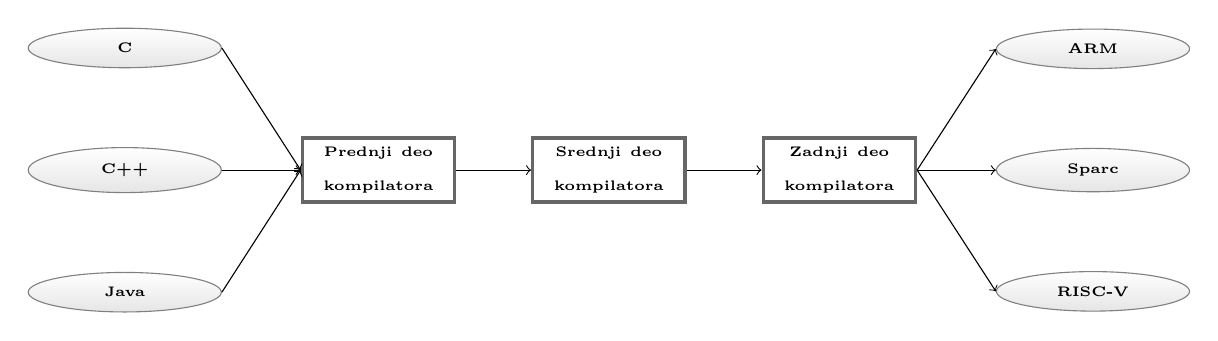
\begin{tikzpicture}[
 roundnode/.style={circle, draw=black!60, fill=white!5, very thick, minimum size=7mm, text width=1cm, align=center},
 squarednode/.style={rectangle, draw=black!60, fill=white!5, very thick, minimum size=5mm, text width=1.7cm, align=center, node distance=0.95cm}
 ]
 
 %Nodes
 \node[squarednode]      (prednji_node)  {\tiny \textbf{Prednji deo kompilatora}};
 \node[squarednode]      (srednji_node)       [right=of prednji_node] {\tiny \textbf{Srednji deo kompilatora}};
 \node[squarednode]      (zadnji_node)       [right=of srednji_node] {\tiny \textbf{Zadnji deo kompilatora}};

 \node[ellismall]        (sparc_node)       [right=of zadnji_node] {\tiny\textbf{Sparc}};
 \node[ellismall]        (arm_node)       [above=of sparc_node] {\tiny\textbf{ARM}};
 \node[ellismall]        (riscv_node)       [below=of sparc_node] {\tiny\textbf{RISC-V}};

 \node[ellismall]        (c++_node)       [left=of prednji_node] {\tiny\textbf{C++}};
 \node[ellismall]        (c_node)       [above=of c++_node] {\tiny\textbf{C}};
 \node[ellismall]        (java_node)       [below=of c++_node] {\tiny\textbf{Java}};

 %Lines
 \draw[->] (prednji_node.east) -- (srednji_node.west);
 \draw[->] (srednji_node.east) -- (zadnji_node.west);
 \draw[->] (zadnji_node.east) -- (arm_node.west);
 \draw[->] (zadnji_node.east) -- (sparc_node.west);
 \draw[->] (zadnji_node.east) -- (riscv_node.west);
 \draw[->] (c_node.east) -- (prednji_node.west);
 \draw[->] (c++_node.east) -- (prednji_node.west);
 \draw[->] (java_node.east) -- (prednji_node.west);
 \end{tikzpicture}
\centering
\caption{Arhitektura modernih kompilatora}
\label{tikz:delovi_kompilatora}
\end{figure}

%Zadnji deo kompilatora...
Zadnji deo kompilatora (eng. \textit{back end}) zavisi od ciljne arhitekture i zadužen je za 
generisanje koda za ciljnu arhitekturu. Generisanje koda podrazumeva transliranje transformisanog međukoda u izlazni 
jezik, obično mašinski jezik računarskog sistema. Ovo uključuje odluke vezane 
za resurse i skladištenje podataka, kao na primer koje promenljive će biti u 
registrima a koje u memoriji, i izbor i određivanje redosleda instrukcija 
zajedno sa odgovarajućim tipovima adresiranja. Takođe, potrebno je generisati i podatke za dabagovanje kako bi se omogućilo debagovanje izvornog programa.

Zadnji deo kompilatora je odgovoran i za sprovođenje mašinski zavisnih optimizacija, odnosno optimizacija koje zavise od detalja arhitekture procesora na kojem će se program izvršavati. Mašinski zavisne optimizacije obuhvataju, na primer, prepisivanje kraćih nizova instrukcije u odgovarajuće efikasnije instrukcije.



Za generisanje mašinskog koda potrebni su samo prednji i zadnji deo kompilatora. Optimizator odnosno srednji deo kompilatora je opcioni i nastao je iz potrebe da dobijeni kôd ima dobre performanse. Svaki dobar kompilator ga sadrži i on predstavlja njegovu najveću komponentu.

% ------------------------------------------------------------------------------
\section{Kompilatorske optimizacije}
\label{sec:compiler_optimization}
% ------------------------------------------------------------------------------ 
Kompilator sprovodi optimizacije sa ciljem povećanja performansi krajnjeg izvršivog koda. Uslov koji svaka optimizacija mora da zadovolji jeste da se optimizovani k\^od ponaša semantički ekvivalentno originalnom kodu. Performanse mogu da se odnose na vreme izvršavanja programa, memorijski prostor potreban prilikom njegovog izvršavanja, memorijski prostor potreban za skladištenje izvršive datoteke ili na energetsku efikasnost programa. 

Kompilatorske optimizacije mogu biti nezavisne ili zavisne od ciljne arhitekture. Nezavisne optimizacije rade za sve ciljne arhitekture i najčešće smanjuju ukupan broj operacija koje treba izvršiti. Zavisne optimizacije koriste detalje arhitekture kako bi povećale performanse. To podrazumeva korišćenje instrukcija koje obavljaju više operacija u isto vreme, imaju kraći zapis ili rade brže od odgovarajućih instrukcija u izvornom kodu. Na primer, na arhitekturi
\texttt{x86-64} se često instrukcija \texttt{mov eax, 0} zamenjuje instrukcijom \texttt{xor eax, eax}.

%!!!!!!!
Optimizacije se u odnosu na opseg koda koji obrađuju mogu podeliti na: lokalne 
optimizacije, globalne optimizacije i međuproceduralne optimizacije.
Lokalne optimizacije rade na nivou jednog osnovnog bloka (eng. \textit{basic block}) i predstavljaju najjednostavnije optimizacije. Globalne optimizacije operišu na nivou pojedinačnih funkcija. Većina lokalnih optimizacija se može modifikovati da radi globalno. Međuproceduralne optimizacije rade na nivou čitavog programa. One istovremeno obrađuju više funkcija od kojih neke mogu biti i u različitim jedinicama prevođenja.

Neke od popularnih optimizacija su umetanje koda (eng. \textit{inlining}), eliminacija mrtvog koda (eng. \textit{dead code elimination}), sažimanje konstanti (eng. \textit{constant folding}), propagiranje konstanti (eng. \textit{constant propagation}), razmotavanje petlji (eng. \textit{loop unrolling}) i neke vrste automatske paralelizacije. U nastavku će samo neke od navedenih optimizacija biti opisane.

% Opis ovih optimizacija moze i da se izostavi...
\begin{description}
    \item[Umetanje koda] (eng. \textit{inlining}) se koristi jer su pozivi funkcija skupa operacija zbog toga što menjaju kontrolu toka izvršavanja i zahtevaju dodatne instrukcije za čuvanje i učitavanje vrednosti registara. Iz tog razloga je poželjno pozive kratkih funkcija zameniti njihovom definicijom. Time se izbegava cena poziva o trošku veće količine memorije za čuvanje programa.
    \item[Razmotavanje petlji] (eng. \textit{loop unrolling}) podrazumeva da se telo petlje ponovi više puta u jednoj iteraciji i da se broj iteracija samim tim isti broj puta smanji. Izvršavanje petlji sa kratkim telom dovodi do velikog broja skokova u kratkom vremenskom intervalu. Skokovi su skupa instrukcija i njihovim smanjenjem moguće je znatno povećati performanse programa. Ovo je moguće samo u posebnim situacijama kada kompilator ima dovoljno informacija o načinu izvršavanja petlje.

    \item[Eliminacija mrtvog koda] (eng. \textit{dead code elimination}) podrazumeva uklanjanje dela programa za koga je statičkom analizom utvrđeno da se nikada neće izvršiti. Brisanjem takvog koda može se uštedeti memorija i ubrzati proces kompilacije. Takođe, ovom tehnikom je, zbog bolje organizacije keš memorije, moguće ubrzati i vreme izvršavanja programa.
\end{description}

Postoji više različitih nivoa optimizacija koji se mogu pokrenuti prilikom poziva kompilatora. Izbor nivoa optimizacije i efekat optimizacija su drugačiji na različitim kompilatorima. Na primer, kompilatori \texttt{gcc} i \texttt{Clang} omogućavaju korisniku da izabere nivo optimizacije tako što kompilatoru prosledi opciju \texttt{-O} iza koje sledi neki od karaktera \texttt{0}, \texttt{1}, \texttt{2}, \texttt{3} ili \texttt{s}. 

Opcijom \texttt{-O0} se naglašava da k\^od nije potrebno optimizovati. Ova opcija je podrazumevana ukoliko nijedan druga opcija nije navedena. Opcije \texttt{-O1} i \texttt{-O2} uključuju redom sve veći broj optimizacija, ali ne povećevaju drastično veličinu memorije koju program koristi prilikom izvršavanja. Opcija \texttt{-O3} predstavlja najveći nivo optimizacije posvećen smanjenju vremena izvršavanja programa. Sa druge strane \textit{-Os} nivo podrazumeva optimizacije koje smanjuju memorijsko zauzeće, ali povećavaju vreme izvršavanja. 

Svaki od opisanih nivoa optimizacija ima svoju konkretnu primenu. Na primer, nivo -O0 se koristi za pravljenje \texttt{debug} verzija programa. Isporučene verzije programa se često kompiliraju navođenjem opcije -O3, dok se nivo -Os koristi za uređaje sa ugrađenim računarom (eng. \textit{embedded devices}).

% ------------------------------------------------------------------------------
\section{Kompilatorska infrastruktura LLVM}
% ------------------------------------------------------------------------------
Projekat LLVM \cite{llvm} je započet kao istraživački projekat 2000. godine na Univerzitetu 
Ilinois od strane Krisa Latnera, čoveka koga je ovaj projekat i proslavio, a koji danas radi na razvoju programskog jezika Mojo \cite{mojo}. Cilj projekta LLVM je bio proučavanje tehnika statičkog i dinamičkog prevođenja proizvoljnih programskih jezika korišćenjem kompiliranja u SSA obliku (eng. \textit{Static Single Assignment}). Naziv LLVM je predstavljao akronim za „virtuelna 
mašina niskog nivoa” (eng. \textit{Low Level Virtual Machine}). Međutim, isti akronim se 
više ne koristi, ali je ime projekta ostalo nepromenjeno. Danas, projekat 
sadrži veliki broj biblioteka i alata koji se koriste kako u komercijalne svrhe 
tako i u svrhe razvoja projekata otvorenog koda. Svaki deo projekta je 
dizajniran kao biblioteka tako da se može ponovo upotrebiti za implementiranje 
drugih alata. Celokupan izvorni kôd je javno dostupan na servisu \href{https://github.com/llvm/llvm-project}{GitHub} i oko njega je 
formirana velika zajednica ljudi koji rade na različitim delovima projekta i 
svakodnevno ga unapređuju. Veliki broj kompanija koristi svoje verzije 
kompilatora LLVM bilo u celosti bilo samo neke njegove delove (prednji, srednji 
ili zadnji deo kimpilatora) za podršku neke procesorkse arhitekture ili kao 
osnovu za novi programski jezik. 

O popularnosti projekta LLVM govori i činjenica da je 2012. godine projekat osvojio nagradu 
\textit{ACM Software System Award} \cite{acm} (nagrada se dodeljuje jednom softverskom sistemu 
godišnje, počevši od 1983. godine), kao i da se dva puta u toku svake godine organizuje \textit{LLVM 
Developers Meeting} i \textit{LLVM WorkShop} u različitim gradovima Evrope i Amerike. Licenca koda u okviru 
LLVM projekta je ”Apache 2.0 License with LLVM exceptions”. Licenciranje se menjalo tokom razvoja 
projekta, ali je projekat uvek bio otvorenog koda.

LLVM se sastoji od velikog broja manjih potprojekata 
koji predstavljaju zasebne i funkcionalne celine. Neki od primarnih potprojekata su 
\href{https://llvm.org/docs/doxygen/group__LLVMCCore.html}{\textit{LLVM Core Libraries}} \cite{llvm_core}, 
\href{https://clang.llvm.org/}{\textit{Clang}} \cite{clang}, 
\href{https://mlir.llvm.org/}{\textit{MLIR}} \cite{mlir}, 
\href{https://openmp.llvm.org/}{\textit{OpenMP}} \cite{openmp}, 
\href{https://polly.llvm.org/}{\textit{polly}} \cite{polly}, 
\href{https://klee-se.org/}{\textit{klee}} \cite{klee}, 
\href{https://lld.llvm.org/}{\textit{LLD}} \cite{llvm_lld}. Svi potprojekti zajedno čine potpun programski prevodilac koji pored 
svog prednjeg, srednjeg i zadnjeg dela poseduje optimizatore, asemblere, linkere i druge alate 
koji pružaju podršku tokom čitavog procesa prevođenja. LLVM implementira i svoj debager koji se 
zove LLDB \cite{lldb}.

Kompilator LLVM je relativno nov u odnosu na druge popularne kompilatore
i prati moderniji dizajn. Za razliku od kompilatora GCC, koji je napisan u
jeziku C i ima monolitnu strukturu, LLVM uživa u pogodnostima koje nudi jezik
C++ pritom koristeći modularnu arhitekturu. Najveći deo projekta je napisan u programskom jeziku C++, ali postoji i interfejs za povezivanje sa jezicima C i Python.
Implementacija kompilatora LLVM prati opštu strukturu kompilatora prikazanu
u poglavlju \ref{sec:kompilatori}. Korake kompilacije izvršavaju različiti alati. Odnos različitih
reprezentacija programa u toku kompilacije i alata koji ga konvertuju iz jedne
reprezantacije u drugu je prikazan na slici \ref{tikz:llvm_interne_reprezentacije}. 
 
U nastavku će redom biti opisani prednji, srednji i zadnji deo kompilatora LLVM sa najvećim fokusom na zadnji deo kompilatora LLVM. Jedno od rešenja koje će u poglavlju \ref{chap:implementacija} biti opisano zahteva dobro poznavanje rada zadnjeg dela kompilatora LLVM, pa je zato ovom delu posvećeno najviše pažnje.

% \begin{figure}
% \includegraphics[width=\textwidth, height=3.5cm]{llvm_arhitektura}
% \caption{Prikaz promena internih reprezentacija programa prilikom prevođenja LLVM kompilatorom}
% \label{fig:llvm_interne_reprezentacije}
% \centering
% \end{figure}

\begin{figure}
    \centering
    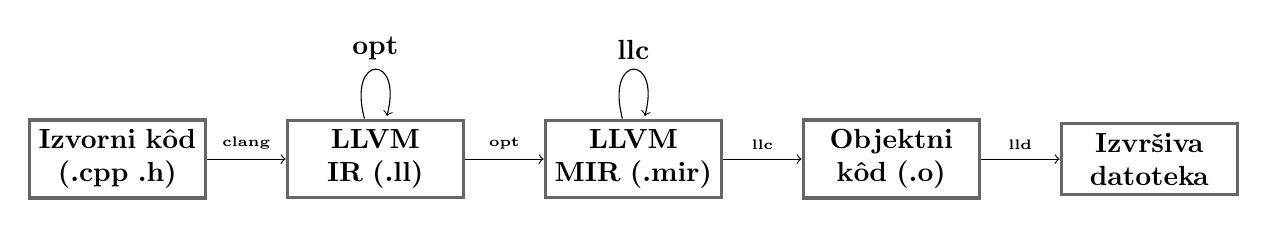
\begin{tikzpicture}[
roundnode/.style={circle, draw=black!60, fill=white!5, very thick, minimum size=7mm},
squarednode/.style={rectangle, draw=black!60, fill=white!5, very thick, minimum size=7mm, text width=2cm, align=center},
][!ht]
\centering
%Nodes
\node[squarednode]      (izvorni_kod_node)  {\textbf{Izvorni k\^od \linebreak (.cpp .h)}};
\node[squarednode]      (llvm_ir_node)       [right=of izvorni_kod_node] {\textbf{LLVM IR (.ll)}};
\node[squarednode]      (llvm_mir_node)       [right=of llvm_ir_node] {\textbf{LLVM MIR (.mir)}};
\node[squarednode]      (objektni_kod_node)       [right=of llvm_mir_node] {\textbf{Objektni k\^od (.o)}};
\node[squarednode]      (izvrsni_fajl_node)       [right=of objektni_kod_node] {\textbf{Izvršiva datoteka}};


%Lines
\draw[->] (izvorni_kod_node.east) -- (llvm_ir_node.west) node[midway, above] {\tiny \textbf{clang}};
\draw[->] (llvm_ir_node.east) -- (llvm_mir_node.west) node[midway, above] {\tiny \textbf{opt}};
\draw[->] (llvm_mir_node.east) -- (objektni_kod_node.west) node[midway, above] {\tiny \textbf{llc}};
\draw[->] (objektni_kod_node.east) -- (izvrsni_fajl_node.west) node[midway, above] {\tiny \textbf{lld}};
% \draw[->] (llvm_ir_node.north) -- (llvm_ir_node.north);
% \draw[->] (llvm_mir_node.north) -- (llvm_mir_node.north);

\path
(llvm_ir_node) edge [loop above] node {\textbf{opt}} (llvm_ir_node)
(llvm_mir_node) edge [loop above] node {\textbf{llc}} (llvm_mir_node);
% (izvorni_kod_node) edge [right] node {clang} (llvm_ir_node)

\end{tikzpicture}
    \caption{Prikaz promena internih reprezentacija programa prilikom prevođenja LLVM kompilatorom}
    \label{tikz:llvm_interne_reprezentacije}
\end{figure}

%Prednji deo LLVM-a!!!!
\subsection{Prednji deo LLVM-a}
Prednji deo LLVM kompilatora je zadužen za pokretanje leksičke, sintaksičke i semantičke analize, kreiranje apstraktnog sintaksnog stabla i na kraju generisanje LLVM međukoda.
Projekat LLVM podržava više različitih prednjih delova kompilatora. Mnoge kompanije takođe razvijaju i održavaju prednje delove kompilatora LLVM za svoje programske jezike. Zahvaljujući tome, LLVM podržava veliki broj programskih jezika kao što su C, C++, Objectve-C, Fortran, Haskell, Swift i drugi. 

Prednji deo kompilatora prilagođen jezicima C i C++ koji su korišćeni u ovom radu jeste Clang. Termin Clang može imati više značenja. Clang može predstavljati prednji deo kompilatora, a takođe može predstavljati i čitav kompilator odnosno alat koji upravlja čitavim procesom kompilacije. U okviru rada, termin Clang će od sada predstavljati prednji deo LLVM kompilatora. 

Funkcija Clang-a je, dakle, da izvorni kôd napisan u jezicima C ili C++ prevede u LLVM međureprezentaciju. Da bi se takvo prevođenje izvelo potrebno je program prvo detaljno izanalizirati, a potom započeti transformacije izvornog koda. U okviru Clang-a sintaksička i semantička analiza su usko povezane. Ukoliko se pronađe greška u bilo kojoj analizi, proces prevođenja se zaustavlja i poruka o razlogu se saopštava korisniku. U suprotnom, obilaskom apstraktnog sintaksnog stabla generiše se LLVM međukod. Ukoliko se program uspešno prevede do međukoda, to znači da je izvorni k\^od ispravan za jezik u kome je napisan. Komanda za prevođenje izvornog C programa u LLVM međureprezentaciju (međukod) je sledeća:
\begin{minted}[breaklines, fontsize=\small]{bash}
clang -S -emit-llvm input.c -o output.ll
\end{minted}

%Srednji deo LLVM-a!!!!
\subsection{Srednji deo LLVM-a}
Srednji deo LLVM kompilatora zadužen je za sprovođenje mašinski nezavisnih optimizacija nad LLVM međureprezentacijom (međukodom) dobijenom od strane \textit{Clang}-a. LLVM međukod je napisan u SSA obliku pogodnom za izvršavanje optimizacija. Optimizacije srednjeg dela LLVM kompilatora su implementirane u vidu prolaza (eng. \textit{pass}). Prolazi implementiraju funkciju \texttt{run} sa argumentima za odgovarajuću jedinicu obrade. Jedinica obrade može biti modul, funkcija ili petlja. Prolazi se dele na analize i transformacije. 

Analize prikupljaju podatke, a transformacije te podatke koriste kako bi izmenile k\^od. 
Transformacije zahtevaju različite vrste analiza koje mogu biti poništene nakon promene koda 
(ukoliko više ne važe). Optimizovanje LLVM međukoda se vrši inkrementalno, tako što međukod dobijen kao rezultat jedne optimizacije postaje ulaz sledećoj optimizaciji. Konačan LLVM međukod zavisi od redosleda izvršavanja optimizacija. Loš redosled može da rezultuje znatno lošijim performansama međukoda, a kasnije i izvršive datoteke.

% Novi LLVM Pass Manager...
% Stari LLVM Pass Manager...
Redosled izvršavanja optimizacionih prolaza određuje LLVM-ov menadžer prolaza (eng. \textit{LLVM Pass Manager}). Menadžer prolaza je takođe odgovoran za upravljanje rezultatima sprovedenih analiza. Rezultati analize bi trebalo da se dele između različitih prolaza kada god je to moguće, budući da je ponovno izračunavanje analiza skupo. Da bi to uradio, LLVM-ov menadžer prolaza mora keširati rezultate analiza ili ih ponovo izračunati u slučaju da su poništeni transformacijama. 

U okviru LLVM kompilatora postoje trenutno dva menadžera prolaza i to stari (eng. \textit{Legacy Pass Manager}) i novi (eng. \textit{New Pass Manager}). Stari menadžer prolaza se koristio dugi niz godina, ali se zbog efikasnosti prešlo na korišćenje novog menadžera. Međutim, i dalje se radi na tome da se sve funkcionalnosti podržane na starom menadžeru implementiraju i na novom. 

Zadatak srednjeg dela LLVM kompilatora obavlja alat \textit{opt}. Alat kao svoje argumente očekuje imena optimizacija koje treba da pokrene i datoteku sa ispravnim LLVM IR kodom koga optimizuje. Primer poziva alata \textit{opt} za pokretanje optimizacionih prolaza \texttt{loweratomic} i \texttt{instnamer} je:

\begin{minted}[breaklines, fontsize=\small]{bash}
opt input.ll -passes="loweratomic,instnamer" -o output.ll
\end{minted}

%Zadnji deo LLVM-a!!!!
\subsection{Zadnji deo LLVM-a}
Zadnji deo kompilatora je odgovoran za generisanje mašinskog koda za ciljnu arhitekturu, ali i mašinski zavisne optimizacije. Poslednja, mašinski zavisna, reprezentacija kroz koju izvorni k\^od prolazi neposredno pre generisanja mašinskog koda se u LLVM terminologiji naziva MIR (eng. \textit{Machine Intermediate Representation}). Instrukcije MIR koda su dosta slične instrukcijama u IR kodu. Međutim, MIR reprezentacija je bliža ciljnoj arhitekturi, te su virtuelni registri zamenjeni pravim fizičkim registrima, a intrukcije MIR koda su stvarno izvršive na konkretnoj arhitekturi. Kompletan pregled jezika dostupan je u okviru dokumentacije projekta LLVM \cite{mir_documentation}.

Prevođenje reprezentacije programa sa mašinski nezavisne na mašinski zavisnu reprezentaciju predstavlja vrlo kompleksan korak koji se naziva izbor instrukcija (eng. \textit{instruction selection}). U okviru LLVM-a postoje tri implementacije izbora instrukcija i to su: \texttt{SelectionDag}, \texttt{GlobalIsel} i \texttt{FastIsel}.

\begin{description}
\item[\textbf{SelectionDAG}] predstavlja podrazumevanu implementaciju izbora instrukcija za većinu procesorskih arhitektura koja koristi grafovsku reprezantaciju programa i algoritme za uparivanje čvorova i različite vrste obilaska grafa.

\item[\textbf{GlobalIsel}] predstavlja novu implementaciju izbora instrukcija sa modularnim dizajnom,
poboljšanim performansama i mogućnošću da optimizuje veći deo kôda. 
Implementacija \texttt{GlobalIsel} nije u potpunosti završena, ali postoji plan inženjera okupljenih oko LLVM-a da ovaj izbor instrukcija zameni \texttt{SelectionDAG}.

\item[\textbf{FastIsel}] je pristup izboru instrukcija koji radi veoma brzo, ali generiše neoptimizovan k\^od. Takođe, postoje instrukcije čije spuštanje nije podržano \texttt{FastIsel} pristupom. 
\end{description}
Rešenja koja će u ovom radu biti predstavljena se oslanjaju na izbor instrukcija \texttt{SelectionDAG} zbog njegove stabilnosti i daleko veće korišćenosti u vreme pisanja rada.
Pristup \texttt{SelectionDAG} je dobio ime po načinu reprezentacije koda za
vreme izbora instrukcija. Naime, osnovni blokovi programa bivaju predstavljeni usmerenim acikličkim grafovima (eng. \textit{directed acyclic graphs}). Čvorovi tog grafa su instrukcije koje imaju tip \texttt{SDNode}, a grane predstavljaju različite zavisnosti koje postoje između instrukcija. Argumentima instrukcija se dodeljuje tip \texttt{SDValue}. Od svih čvorova u grafu posebno se izdvajaju dva i to su ulazni čvor i koren. Ulazni čvor obeležava početak osnovnog bloka i služi samo za postavljanje veza. Sa druge strane, koren označava kraj bloka. Na kraju obrade je vezan za poslednju instrukciju osnovnog bloka.

Pristup \texttt{SelectionDAG}  izboru instrukcija implementaran je pomoću istoimene klase \texttt{SelectionDAG}. Gore pomenuta grafovska reprezentacija programa se gradi prolaskom kroz LLVM međukod uz pomoć klase \texttt{SelectionDAGBuilder}. Za svaku instrukciju se kreira čvor na osnovu operacije koju predstavlja. Veze se kreiraju kada neki čvor
koristi izlaznu vrednost drugog čvora. Tip te vrednosti određuje tip veze. Ovako konstruisan graf nije pogodan za spuštanje instrukcija, te se nad njim moraju izvršiti određene transformacije. 

Graf se optimizuje zamenom grupe povezanih čvorova jednostavnijim grupama korišćenjem algoritama za uparivanje stabala. Optimizacije nad grafom mogu biti i mašinski zavisne i mašinski nezavisne. Takođe, graf može da sadrži nepodržane tipove i operacije za ciljnu arhitekturu. Njih je potrebno zameniti odgovarajućim podržanim tipovima i operacijama i tu transformaciju nazivamo legalizacijom tipova i operacija. Način legalizacije zavisi od arhitekture i implementiran je u odgovarajućim klasama \texttt{TargetLowering}, što znači da za svaku arhitekturu postoju odgovarajuća klasa \texttt{TargetLowering}. Neki od primera klasa \texttt{TargetLowering} su \texttt{ArmTargerLowering}, \texttt{RISCVIselLowering} i \texttt{ARMIselLowering}. Optimizacije i legalizacije se vrše više puta u određenom redosledu i rezultuju grafom spremnim za spuštanje
instrukcija. 

Proces spuštanja instrukcija je prilično jednostavan i zasniva se na uparivanju čvorova. Čvorovi svake \texttt{SelectionDAG} strukture traže svoj pandan za ciljnu arhitekturu. U ovom koraku se ne zamenjuju baš svi čvorovi već neki prolaze u narednu fazu prevođenja.

Poslednja stvar koju je potrebno eliminisati iz LLVM međukoda su virtuelni registri. Korak u kome se virtuelni registri zamenjuju konkretnim registrima za ciljnu arhitekturu nazivamo dodeljivanjem registara. Neki od fizičkih registara se su već implicitno dodeljeni na osnovu instrukcija. Preostali registri se dodeljuju korišćenjem heuristika, jer je problem NP-kompletan, pa za njega ne možemo koristiti optimalan algoritam. Jedna od često korišćenih heuristika je gramziva (eng. \textit{greedy}) koja prednost prilikom dodeljivanju registara daje promenljivama sa dužim životnim vekom. 

Optimizacioni prolazi postoje i na MIR nivou i način njihovog izvršavanja je sličan prolazima na IR nivou odnosno na nivou mašinski nezavisnog međukoda. Međutim, optimizacije na MIR nivou su vezane za ciljnu arhitekturu. Mašinski zavisni prolazi nasleđuju klasu \texttt{MachineFunctionPass} i implementiraju funkciju \texttt{runOnMachineFunction} koja se poziva za svaku funkciju u izvornom kodu. Prolazi se izvršavaju iterativno u unapred zadatom redosledu.

Poslednji prolaz na MIR kodu u kome se, u zavisnosti od navedenih opcija, emituje asemblerski ili objektni k\^od za ciljnu arhitekturu i kojim se završava zadatak kompilatora jeste \texttt{AsmPrinter}. Ukoliko je emitovan asemblerski k\^od on se prevodi do objektnog koda korišćenjem asemblera, dok se objektni kôd povezuje sa sistemskim i korisničkim bibliotekama i drugim objektnim datotekama pomoću povezivača (eng. \textit{linker}) kako bi se od njega dobila krajnja izvršiva datoteka.

Posao zadnjeg dela LLVM kompilatora obavlja alat \texttt{llc}. Alatu se opciono zadaje
vrsta izlaza koju treba da generiše i nivo optimizacije. Izlaz alata \texttt{llc} može biti asemblerski ili objektni k\^od. Još jedan bitan parametar koji se alatu \texttt{llc} može proslediti je ciljna arhitektura. Ciljna arhitektura se zadaje argumentom \texttt{-mtriple} i vrednošću u vidu niske koja sadrži naziv arhitekture procesora, njegovog proizvođača, operativnog sistema i okruženja. Komanda za prevođenje LLVM međukoda do objektnog koda za
arhitekturu \texttt{x86\_64} i operativni sistem \texttt{Linux} je sledeća:

\begin{minted}[breaklines, fontsize=\small]{bash}
llc -filetype=obj -mtriple="x86_64-unknown-linux-gnu" input.ll -o output.o 
\end{minted}

% ------------------------------------------------------------------------------
\section{LLVM međureprezentacija}
\label{sec:llvm_ir}
% ------------------------------------------------------------------------------
%U ovoj sekciji će detaljnije biti objašnjena sintaksa LLVM međurerezentacije i način na koji je ona podržana u okviru projekta LLVM. Diskusija o LLVM međureprezentaciji navedena je kako bi kasnije poglavlje koje se tiče implemetacije rešenja bilo razumljivije.

%Prednji deo LLVM kompilatora je zadužen da izvorni k\^od prevede u LLVM mašinski nezavisan međukod. 
Da bi kompilator mogao da prevodi više programskih jezika za više ciljnih arhitektura potrebno je da međukod bude na dovoljno apstraktnom nivou da ne zavisi od procesorske arhitekture, ali i na dovoljno opštem nivou kako ne bi zavisio od programskog jezika u kome je izvorni k\^od napisan. LLVM međukod je zapisan u SSA obliku što znači da poštuje svojstvo jedinstvenog statičkog dodeljivanja. Ovo svojstvo omogućava da se svakoj promenljivoj samo jednom može dodeliti vrednost i da svakoj upotrebi promenljive prethodi njena definicija. 

Datoteke koje u sebi sadrže LLVM međukod se najčešće obeležavaju ekstenzijom \texttt{.ll}. Na početku takvih datoteka se nalazi ime datoteke u kojoj je napisan izvorni kôd (npr. \texttt{test.c}), informacije o načinu zapisa podataka i naziv ciljne arhitekture. U nastavku se nalaze globalne promenljive i funkcije čiji nazivi počinju prefiksom ’@’.

LLVM međureprezentacija (LLVM IR) je u okviru projekta LLVM implementirana kroz hijerarhiju klasa. Svaka od klasa u toj hijerarhiji predstavlja jedan od sledećih entiteta: modul, funkciju, osnovni blok i instrukciju. U nastavku će svaki od entiteta biti pojedinačno objašnjen.

Moduli su najviši entiteti u hijerarhiji i definisani su sadržajem datoteka u kojima se nalazi LLVM međureprezentacija (LLVM međukod). Funkcije izgrađuju jedan modul i odgovaraju funkcijama napisanim u izvornom kodu. Svaka funkcija se sastoji od niza osnovnih blokova, a svaki blok od niza instrukcija. Lokalne promenljive funkcija su predstavljene virtuelnim registrima. Identifikatori virtuelnih registara počinju karakterom ’\%’. Zahvaljujući SSA obliku, svakom od virtuelnih registara se vrednost može dodeliti tačno jednom, tako da virtuelnih registara može biti neograničeno mnogo.

Osnovni blokovi (eng. \textit{basic blocks}) predstavljaju niz instrukcija koji se uvek izvršavaju linearno i u celini. Svaka funkcija započinje prvim osnovnim blokom i završava se poslednjim osnovnim blokom. Ukoliko se nekim programskim tokom uđe u osnovni blok on će se uvek izvršiti do kraja. To implicira da se instrukcije grananja pojavljuju isključivo na krajevima osnovnih blokova. Granice osnovnih blokova su označene poput labela u asemblerskom jeziku.

Na kraju, instrukcije izgrađuju osnovne blokove i delom odgovaraju instrukcijama u izvornom kodu. Instrukcije LLVM međukoda mogu biti dvoadresne ili troadresne što podrazumeva da svaka instrukcija ima jedan ili dva argumenta koji predstavljaju operande i dodatni argument koji predstavlja lokaciju za smeštanje rezultata. 
Instrukcije se sastoje od naziva (\texttt{alloca}, \texttt{store}, \texttt{zext}, ...), tipa (\texttt{i8}, \texttt{i16}, \texttt{float}, ...) i operanada. Dodatne informacije o instrukcijama i globalnim objektima se čuvaju u vidu metapodataka. Metapodaci počinju karakterom ’!’ i obično se koriste kao informacije za debagovanje. Primer LLVM međukoda dobijenog od kratkog programa napisanog u programskom jeziku C prikazan je u listingu \ref{llvm_ir}, dok je program od koga je LLVM međukod dobijen prikazan u 
listingu \ref{short_c}. 

\begin{listing}
\begin{minted}[breaklines, fontsize=\small]{C++}
#include <stdio.h>

int main() {
    int x;
    scanf("%d", &x);
    if (x > 0)
        printf("Welcome to the LLVM IR!");
    
    return 0;
}
\end{minted}
\caption{Kratak C program na osnovu koga kreiramo program sa LLVM međukodom}
\label{short_c}
\end{listing}

\begin{listing}
\begin{minted}[fontsize=\footnotesize,breaklines]{llvm}
; ModuleID = 'test.c'
source_filename = "test.c"
target datalayout = "e-m:e-p270:32:32-p271:32:32-p272:64:64-i64:64-f80:128-n8:16:32:64-S128"
target triple = "x86_64-pc-linux-gnu"

@.str = private unnamed_addr constant [3 x i8] c"%d\00", align 1
@.str.1 = private unnamed_addr constant [24 x i8] c"Welcome to the LLVM IR!\00", align 1

; Function Attrs: noinline nounwind optnone uwtable
define dso_local i32 @main() #0 {
  %1 = alloca i32, align 4
  %2 = alloca i32, align 4
  store i32 0, i32* %1, align 4
  %3 = call i32 (i8*, ...) @__isoc99_scanf(i8* noundef getelementptr inbounds ([3 x i8], [3 x i8]* @.str, i64 0, i64 0), i32* noundef %2)
  %4 = load i32, i32* %2, align 4
  %5 = icmp sgt i32 %4, 0
  br i1 %5, label %6, label %8

6:                                                ; preds = %0
  %7 = call i32 (i8*, ...) @printf(i8* noundef getelementptr inbounds ([24 x i8], [24 x i8]* @.str.1, i64 0, i64 0))
  br label %8

8:                                                ; preds = %6, %0
  ret i32 0
}

declare i32 @__isoc99_scanf(i8* noundef, ...) #1

declare i32 @printf(i8* noundef, ...) #1

attributes #0 = { noinline nounwind optnone uwtable "frame-pointer"="all" "min-legal-vector-width"="0" "no-trapping-math"="true" "stack-protector-buffer-size"="8" "target-cpu"="x86-64" "target-features"="+cx8,+fxsr,+mmx,+sse,+sse2,+x87" "tune-cpu"="generic" }
attributes #1 = { "frame-pointer"="all" "no-trapping-math"="true" "stack-protector-buffer-size"="8" "target-cpu"="x86-64" "target-features"="+cx8,+fxsr,+mmx,+sse,+sse2,+x87" "tune-cpu"="generic" }

!llvm.module.flags = !{!0, !1, !2, !3, !4}
!llvm.ident = !{!5}

!0 = !{i32 1, !"wchar_size", i32 4}
!1 = !{i32 7, !"PIC Level", i32 2}
!2 = !{i32 7, !"PIE Level", i32 2}
!3 = !{i32 7, !"uwtable", i32 1}
!4 = !{i32 7, !"frame-pointer", i32 2}
!5 = !{!"Ubuntu clang version 14.0.0-1ubuntu1.1"}
\end{minted}
\caption{Primer LLVM međureprezentacije (LLVM međukoda)}
\label{llvm_ir}
\end{listing}

Novitet koji se uvodi na nivou LLVM međureprezentacije, a koji ne postoji na nivou izvornog koda, jeste intrinzička funkcija. Intrinzička funkcija (eng. \textit{intrinsic function}) predstavlja funkciju koja se kroz veći deo prevođenja LLVM kompilatorom (eng. \textit{LLVM pipeline}) može smatrati validnom iako nikakav k\^od ne postoji iza nje, ali koja će u određenjom trenutku biti zamanjena blokom koda koji bi trebalo da predstavlja. Da bi neka funkcija mogla biti smatrana intrinzičkom funkcijom, potrebno je istu deklarisati u okviru posebnih datoteka projekta LLVM. To su datoteke sa ekstenzijom \texttt{.td} čiji je sadržaj napisan jezikom \texttt{TableGen}.

\texttt{TableGen} predstavlja domenski specifičan jezik (eng.~\textit{domain specific language}) razvijen za potrebe LLVM projekta koji je zadužen za generisanje različitih datoteka ili struktura podataka u situacijama kada je manuelno kreiranje i održavanje istih dosta zahtevno. \texttt{TableGen} datoteke pokrivaju značajan procenat celokupnog koda u okviru LLVM projekta. Pozovom alata \texttt{cloc} (eng. \textit{count lines of code}) koji je u stanju da prebroji linije u datoteci i kategorizuje ih prema programskom jeziku dobija se da je više od 500 000 linija koda projekta LLVM napisano upravo u sintaksi \texttt{TableGen}. 

% ------------------------------------------------------------------------------
\section{LLVM infrastruktura za testiranje}
% ------------------------------------------------------------------------------

Za testiranje promena napravljenih u okviru projekta LLVM kreirana je čitava infrastruktura za testiranje. LLVM infrastruktura za testiranje omogućava korišćenje testova jedinica koda (eng. \textit{unit tests}) kao i čitavih programa za testiranje. Dodatno, posebna vrsta testova su i regresioni testovi koji služe da obezbede da promene napravljene u LLVM projektu neće izazvati defekte u njegovoj funkcionalnosti. Testovi jedinica koda i regresioni testovi su sadržani u LLVM-ovom repozitorijumu.
%u okviru direktorijuma \texttt{llvm/test} i \texttt{llvm/unittests}. 
Očekuje se da se u svakom trenutku svaki od ovih testova izvršava sa očekivanim ishodom i preporuka je pokrenuti ih pre i nakon kreiranja promena na projektu.

%Ovaj deo moze i da se izostavi...
\paragraph{Testovi jedinica koda} su napisani korišćenjem \textit{Google} testova i \textit{Google Mock}-a i nalaze se u direktorijumu \texttt{llvm/unittests}. Testovi jedinica koda se koriste za proveru korišćenja biblioteka i za druge generičke strukture podataka. Ukoliko je potrebno 
testirati transformacije i analize sprovedene na nivou međureprezentacije, odnosno IR nivou, u tom slučaju je bolje koristiti regresione testove.


\paragraph{Čitavi programi za testiranje} se nazivaju "LLVM test suite" ili samo "test-suite" i za njih postoji repozitorijum na platformi \texttt{GitHub}. 
Ovi testovi sadrže delove koda koji predstavljaju čitave programe i koji se mogu sastaviti i povezati u samostalan program koji se može izvršiti. Programi se obično pišu u jezicima visokog nivoa kao što su C ili C++.
Programi za testiranje se prevode korišćenjem odabranih parametara kompilatora, a zatim se izvršavaju kako bi se uhvatile informacije o njegovom izlazu i vremenu izvršavanja. Izlaz programa za testiranje se poredi sa referentnim izlazom. Za više detalja pogledajte \href{https://www.llvm.org/docs/TestSuiteGuide.html}{\textit{test-suite} vodič} \cite{test_suite}.

\subsection{Regresioni testovi}
{Regresioni testovi} su mali delovi koda koji testiraju specifičnu komponentu LLVM kompilatora ili izazivaju određenu grešku u okviru LLVM-a. Jezik u kome su napisani zavisi od dela LLVM-a koji se tim testom proverava. 
Kada se pronađe neka greška u okviru projekta LLVM, obično se na osnovu nje kreiraju regresioni testovi koji sadrže taman dovoljno koda da reprodukuju problem. %Kreirane regresione testove bi trebalo smestiti u okviru \texttt{llvm/test} direktorijuma. 
Na primer, regresioni test može biti mali deo LLVM IR koda izdvojen iz neke aplikacije. %ili \texttt{benchmark} statistika.
Regresioni testovi se nalaze u okviru direktorijuma \texttt{llvm/test}.
Promene opisane u ovom radu biće testirane kreiranjem regresionih testova, a potom pokretanjem alata \texttt{llvm-lit} \cite{lit} i \texttt{Filecheck} \cite{filecheck} nad njima.

%\begin{description}
%\item[Alat \texttt{llvm-lit}] 
\paragraph{Alat \texttt{llvm-lit}} je deo projekta LLVM.  To je alat za izvršavanje LLVM i Clang programa za testiranje, sumiranje njihovih rezultata i saopštavanje potencijalnih grešaka. Alat je dizajniran tako da bude lak za testiranje (u smislu memorijskog zauzeća i minimalističke sintakse) sa što jednostavnijim korisničkim interfejsom. Alat je moguće pokrenuti nad jednim ili više testova navedenih u komandnoj liniji. Testovi mogu biti ili pojedinačne test datoteke ili direktorijumi sa test datotekama. Svaki navedeni test se izvršava, nekada i konkurentno. Kada su svi testovi pokrenuti \texttt{llvm-lit} počinje sa štampanjem informacija o broju testova koji su uspešno završili sa radom i onima kod kojih se desila greška.

%\item[Alat \texttt{Filecheck}]  
\paragraph{Alat \texttt{Filecheck}} čita dve datoteke (jednu sa standardnog ulaza, a jednu navedenu kao argument komandne linije) i koristi jednu kako bi verifikovao drugu. Ovakvo ponašanje je izuzetno korisno za pokretanje skupova testova, kojima se proverava da li rezultat rada nekog alata (na primer, alata \texttt{llc}) sadrži neku očekivanu informaciju (na primer, instrukciju \texttt{clmul} u asemblerskom kodu koji alat generiše). Deluje da je alat \texttt{Filecheck} vrlo sličan alatu \texttt{grep}, međutim alat \texttt{Filecheck} omogućava daleko efikasnije prepoznavanje više različitih ulaza u jednoj datoteci i izlistavanje prepoznatih delova u specifičnom redosledu. Uputstvo za korišćenje alata \texttt{Filecheck} prikazano je u listingu \ref{file_check}. Datoteka \texttt{match-filename} predstavlja datoteku koja sadrži obrazac koji treba prepoznati. Datoteka koja se verifkuje se unosi sa standardnog ulaza ukoliko opcija \texttt{--input-file} nije upotrebljena.

%\end{description}

% Alat Filecheck...

\begin{listing}[!ht]
\begin{minted}[breaklines, fontsize=\small]{bash}
FileCheck match-filename [–check-prefix=XXX] [–strict-whitespace]
\end{minted}
\caption{Uputstvo za pokretanje alata \texttt{FileCheck}}
\label{file_check}
\end{listing}




% ------------------------------------------------------------------------------
\chapter{Algoritam CRC i problem njegovog prepoznavanja}
\label{chap:crc}

Sa porastom protoka podataka kroz različite mrežne kanale, greške u podacima odnosno narušavanje 
njihovog integriteta je postalo sve učestalije. Usled unutrašnjih ili spoljašnjih 
smetnji, podaci koji se prenose često postaju korumpirani ili oštećeni. To dovodi do gubitka 
podataka. Jedna od najpoznatijih metoda za otkrivanje oštećenja u podacima je 
ciklična provera redundansi (eng. \textit{Cyclic Redundancy Check - CRC}), odnosno algoritam CRC.


% Primene CRC algoritama...
Primene algoritma CRC obuhvataju različite aspekte digitalne komunikacije. Na primer, u mrežnim protokolima kao što je \texttt{Ethernet} \cite{ethernet_protocol} algoritam CRC se koristi za otkrivanje grešaka prilikom prenosa podataka. U bežičnoj komunikaciji, na primer tehnologiji \texttt{Bluetooth} \cite{bluetooth}, algoritam CRC se primenjuje kako bi se osigurala tačnost i pouzdanost prenosa podataka između uređaja. Takođe, u sistemu za čuvanje podataka kao što je \texttt{RAID} (eng. \textit{Redundant Array of Independent Disks}) \cite{raid}, CRC može 
otkriti i ispraviti greške na nivou diska.

\section{Algoritam CRC}
% ------------------------------------------------------------------------------

Ciklična provera redundansi predstavlja tehniku koja omogućava da se putem dodatnih bitova detektuju promene u podacima. Ova tehnika se u velikoj meri koristi u digitalnim mrežama i u uređajima za skladištenje. Podaci koji ulaze u ove sisteme se proširuju dodatnim bitovima (dodatni bitovi se nadovezuju na bitove podataka). Dodatne bitove nazivamo kontrolnim bitovima (eng. \textit{checksum}) i oni se dobijaju kao ostatak pri deljenju bitova podataka sa odabranim polinomom. Deljenje se izvodi u binarnoj osnovi. Po prijemu podataka, izračunavanje se ponavlja (deljenje bitova podataka odabranim polinomom) i ukoliko se dobijena vrednost ne poklapa se očekivanom vrednošću, zaključuje se da je došlo do narušavanja integriteta podataka i mogu se pokrenuti akcije za ispravljanje oštećenih delova podataka. % Dakle, algoritam CRC se može koristiti i za korekciju podataka.

Algoritam CRC se tako naziva jer su bitovi kojima se podaci proširuju redundantni (njima se podaci samo proširuju), a sam algoritam se zasniva na cikličnim kodovima \cite{cyclic_codes}. Algoritam CRC je popularan jer se može implementirati u samom hardveru, lako se matematički analizira i naročito dobro detektuje greške nastale usled šuma, a unutar transportnih kanala. % Pošto kontrolni bitovi imaju fiksiranu dužinu, funkcija koja ih generiše se obično naziva i heš funkcija.

%footnote[1]{Ciklični kodovi su blokovi koda (bitova) takvi da ciklično pomeranje svake ispravne kodne reči daju drugu ispravnu kodnu reč. Ciklični kodovi se koriste za korekciju grešaka zbog svojih algebarskih svojstva koja omogućavaju efikasno otkrivanje i ispravljanje grešaka.}

Specifikacija CRC koda zahteva i definiciju polinoma generatora. Polinom generator postaje delilac u polinomskom deljenju, a poruka se uzima kao deljenik. Količnik pri deljenju se odbacuje, a bitovi ostatka se uzimaju kao kontrolni bitovi. Bitno je naglasiti da se koeficijenti polinoma računaju na osnovu aritmetike u konačnom polju. U praksi, sve često korišćene verzije algortima CRC koriste konačno polje sa dva elementa (odnosno Galoavu grupu GF(2)). 
%Ovo polje omogućava da se operacija sabiranja može sprovesti bitovski paralelno (bez prenosa između cifara). 

% Mislim da je ovaj deo bitan i voleo bih da ga zadrzim u radu.
Najjednostavniji metod za detekciju grešaka u podacima jeste bit parnosti, koji predstavlja kontrolni CRC bit dužine jedan. Bit parnosti koristi polinom $x+1$ (dva člana) i obično se označava kao \texttt{CRC-1}. Ovaj kontrolni bit ima vrednost jedan ukoliko je broj jedinica u bitovima podataka paran. U suprotnom, ovaj kontrolni bit ima vrednost 0. Primalac poruke proširene bitom parnosti proverava da li vrednost bita parnosti odgovara parnosti bitova poruke. Ukoliko dođe do promene u podacima koja se ne odrazi na parnost bitova, ta promena neće biti detektovana ovom metodom.

Sledeći jednostavan metod za detekciju grešaka jeste izračunavanje sume bitova podataka. Bitovi sume se nadovezuju na bitove podataka (odnosno dodeljuju podacima u vidu kontrolnih bitova) i podaci se u tom obliku šalju. Primalac poruke (odnosno podatka) može po prijemu poruke izračunati njenu sumu bitova i tu vrednost uporediti sa vrednošću predstavljenom kontrolnim bitovima. Ukoliko se ove dve sume razlikuju to bi trebalo da signalizira da je usled transfera podatka 
došlo do narušavanja njegovog integriteta. U suprotnom, ukoliko su sume identične, to 
bi značilo da do narušavanja integriteta podataka nije došlo.
Međutim, ukoliko su bitovi podataka promenjeni, 
ali tako da je suma njihovih bitova ostala ista, upoređivanjem sume bitova poruke i 
kontrolnih bitovima dolazi se do zaključka da se sa primljenom 
porukom ništa nije desilo iako zapravo jeste. Takođe, ukoliko je neki od kontrolnih bitova promenjen, dolazi se do zaključka da je integritet poruke narušen iako zapravo nije. 

Navedeni primeri govore o tome da je izbor polinoma generatora zapravo najvažniji deo implementacije algoritma CRC. Polinom mora biti izabran tako da se maksimizuju mogućnosti otkrivanja grešaka uz minimizovanje ukupnih verovatnoća kolizije. Pod kolizijom se podrazumevaju opisane situacije u kojima promena u podacima nije detektovana (a desila se) i situacije u kojima se promena signalizira iako se nije stvarno desila. Najvažniji atribut polinoma jeste njegov najveći stepen zbog njegovog direktnog uticaja na dužinu kontrolnih bitova. 

Kontrolni bitovi dužine \textit{n} nazivaju se \textit{n}-bitnim CRC-om. Za dato \textit{n} moguće je generisati više različitih kontrolnih bitova (svaki za različiti polinom). Polinom sa najvišim stepenom \textit{n} ima ukupno \textit{n+1} članova, samim tim i bitovsku reprezentaciju dužine \textit{n+1}. Najčešće korišćeni polinomi su polinomi dužine 9 bita (\texttt{CRC-8}), 17 bita (\texttt{CRC-16}), 33 bita (\texttt{CRC-32}) i 65 bita (\texttt{CRC-64}). Na primer, često korišćeni polinom u implementaciji algoritma \texttt{CRC-8} jeste $x^8 + x^7 + x^6 + x^4 + x^2 + 1$, dok je u slučaju algoritma \texttt{CRC-16} to polinom $x^{16} + x^{15} + x^2 + 1$. Različite konfiguracije polinoma generatora omogućavaju prilagođavanje algoritma CRC specifičnim zahtevima sistema.

% OPIS PRIMERA BI TREBALO SREDITI...
Pojednostavljen primer računanja CRC kontrolnih bitova na strani pošiljaoca i provere integriteta podataka na strani primaoca poruke prikazan je u listinzima \ref{posiljalac_poruke} i \ref{primalac_poruke}. U primeru se 14-bitna poruka proširuje sa tri 0 bita (inicijalnim kontrolnim bitovima), a kao polinom generator koristi se polinom $x^3 + x + 1$. U listingu \ref{posiljalac_poruke} prikazano je računanje kontrolnih bitova na strani pošiljaoca poruke. Kontrolni bitovi se računaju kao ostatak pri deljenju bitova poruke sa bitovima polinoma. Deljenje se sprovodi primenom ekskluzivne disjunkcije (operacije XOR) i pomeranja bitova polinoma za po jedan bit udesno u svakoj iteraciji. Ostatak dobijen na kraju deljenja predstavlja kontrolne bitove kojima će poruka biti produžena i u tom obliku poslata. 
U listingu \ref{primalac_poruke} prikazana je provera ispravnosti podataka na strani primaoca poruke. Ispravnost primljene poruke se proverava ponovnim izvođenjem deljenja, ovog puta nad bitovima primljene poruke (bitovi poruke i kontrolni bitovi dobijeni iz prethodnog deljenja). Ukoliko je ostatak pri deljenju jednak 0 (odnosno jednak inicijalnim kontrolnim bitovima) zaključuje se da do promene podataka nije došlo. U suprotnom se zaključuje da je do promene podataka došlo.

%Ostatak bi trebao biti jednak 0 odnosno inicijalnim kontrolnim bitovima ako nema grešaka koje se mogu otkriti.

\begin{listing}[!ht]
\begin{minted}[breaklines, fontsize=\small]{bash}
11010011101100 000 <--- bitovi podataka prošireni sa tri inicijalna kontrolna bita
1011               <--- delilac (polinom generator x^3 + x + 1)
01100011101100 000 <--- rezultat
 1011              <--- delilac ...
00111011101100 000
  1011
00010111101100 000
   1011
00000001101100 000 <--- deljenje se nastavlja od prvog sledećeg bita 1
       1011             
00000000110100 000
        1011
00000000011000 000
         1011
00000000001110 000
          1011
00000000000101 000
           101 1
-----------------
00000000000000 100 <--- ostatak (poslednja 3 bita). 
                   Deljenje se zaustavlja pošto je količnik postao 0. 
\end{minted}
\caption{Računanje kontrolnih bitova na strani pošiljaoca}
\label{posiljalac_poruke}
\end{listing}

\begin{listing}[!ht]
\begin{minted}[breaklines, fontsize=\small]{bash}
11010011101100 100 <--- bitovi podataka prošireni kontrolnim bitovima
1011               <--- delilac (polinom generator x^3 + x + 1)
01100011101100 100 <--- rezultat
 1011              <--- delilac ...
00111011101100 100

......

00000000001110 100
          1011
00000000000101 100
           101 1
------------------
00000000000000 000 <--- ostatak
\end{minted}
\caption{Provera integriteta podataka na strani primaoca poruke}
\label{primalac_poruke}
\end{listing}

% Table-based CRC
%Objasniti pojam table-based verzije algoritma CRC...
Prikazani algoritam može biti prilično neefikasan i u najgorem slučaju obrađivati bit 
po bit. Za veće ulazne podatke, to bi bilo prilično sporo. Međutim, moguće je unapred 
izračunati rezultate deljenja za svaku moguću vrednost bloka podataka koji se deli 
polinomom i sačuvati ih u pomoćni niz ili tabelu. Sačuvane rezultate bi potom bilo 
moguće koristiti čime bi se ubrzala obrada. U slučaju polinoma stepena 8 blok podataka 
koji se deli polinomom je dužine 8 bita (jednog bajta). To znači da bi pomoćni niz 
čuvao ukupno 256 vrednosti (za svaku vrednost bajta čuvao bi se po jedan rezultat 
deljenja). Verzije algoritma CRC koje koriste pomoćne nizove odnosno tabele nazivaju 
se \textit{table-based} verzije algoritma CRC.


% ------------------------------------------------------------------------------
\section{Problem prepoznavanja algoritma CRC}
% ------------------------------------------------------------------------------
Problem koji se u ovom radu rešava jeste prepoznavanje (detektovanje) algoritma CRC i 
njegovo optimizovanje. Pod prepoznavanjem se podrazumeva pronalaženje njegove 
implementacije u izvornom kodu nekog programa. % Prepoznavanje i optimizovanje algoritma CRC se sprovodi sa ciljem da se program koji sadrži njegovu implementaciju izvršava efikasnije.
Da bi prepoznavanje algoritma CRC bilo izvodiljivo potrebno je da njegova 
implementacija bude unapred poznata. Prepoznavanje se može izvršiti prolaskom kroz 
k\^od programa (krećući se od prve ka poslednjoj instrukciji ili u obrnutom smeru). 
Ovim postupkom se vrši upoređivanje redosleda instrukcija programa sa redosledom 
instrukcija algoritma CRC. Takođe se proverava da li svaka od instrukcija programa 
sadrži argumente istog tipa i iste vrednosti kao odgovarajuća instrukcija u algoritmu 
CRC. Različit redosled nezavisnih instrukcija programa ne bi trebalo da utiče na 
rezultat prepoznavanja. Korišćenje različitih, funkcionalno ekvivalentnih instrukcija 
u programu takođe ne bi trebalo da utiče na rezultat prepoznavanja. Na kraju ovakvog 
postupka, ukoliko ni u jednoj od spomenutih provera nije bilo razlike između 
očekivanih i dobijenih rezultata, može se zaključiti da je algoritam prepoznat 
(odnosno detektovan). Tek tada se mogu pokrenuti akcije za njegovo optimizovanje.

%Detektovanje odnosno prepoznavanje nekog algoritma moguće je uraditi prolaskom kroz čitav kod algoritma koji se proverava. Ovim postupkom se proverava da li se naredbe algoritma javljaju u redosledu
% Detektovanje odnosno prepoznavanje nekog algoritma moguće je uraditi sprovođenjem 
% čitavog algoritma i upoređivanjem da li se u svakom od koraka izvršava ona 
% naredba ili instrukcija koja se očekuje i proveravanjem da li svaka od 
% promenljivih koje figurišu u algoritmu u svakom trenutku ima očekivanu vrednost. 
% %Takođe, potrebno je doyvoliti različiti raspored nezavisnih instrukcija... 
% Na kraju ovakvog postupka, ukoliko ni u jednoj od spomenutih provera nije bilo razlike između očekivanih i dobijenih rezultata, može se zaključiti da je algoritam detektovan odnosno prepoznat.

Problem sa prepoznavanjem algoritma CRC jeste taj što postoji veliki broj njegovih implementacija, pa je za svaku od njih potrebno napraviti poseban šablon za prepoznavanje (eng. \textit{pattern matcher}). Pod šablonom za prepoznavanje se podrazumevaju sve provere koje se nad jednim programom vrše (prolazak kroz njegove instrukcije, provera njihovog redosleda, vrednosti njihovih operanada i druge) kako bi se ustanovilo da li on u sebi sadrži implementaciju nekog algoritma. 
Razvijanje svakog od šablona zahteva dosta vremena i truda kako bi se napravio šablon sposoban da prepozna što veći broj modifikacija iste verzije algoritma. 
Sa druge strane, prepoznavanje jednostavnijih algoritama ili aritmetičkih izraza (proširenog oblika kvadrata binoma, kuba binoma, izraza za računanje rešenja kvadratne jednačine) je daleko jednostavnije i zahteva pokrivanje znatno manjeg broja slučajeva
\footnote{U okviru \texttt{GitHub} repozitorijuma koji sadrži sav materijal ovog rada nalazi se i implementacija LLVM optimizacionog prolaza pod nazivom \texttt{expression-optimizer}. Svrha tog optimizacionog prolaza jeste detektovanje proširenog oblika kvadrata binoma ($a^2 + 2ab + b^2$) i zamena istog odgovarajućim skrećenim zapisom ($(a + b)^2$).}.
 

Kako se usled porasta broja informacija koje se prosleđuju putem interneta, povećava upotreba algoritma CRC i drugih metoda za proveru integriteta podataka tako raste potreba da svaka od korišćenih metoda bude što efikasnija. Jedan od načina da se obezbedi efikasnost ovih algoritama jeste upravo uvođenje dodatnih provera u prevodiocima kojima bi se ovi algoritmi detektovali i potom optimizovali.

%Trebalo bi napomenuti da je pozeljno koristiti efikasne verzije CRC algoritma i da se iz tog razloga ohrabruje njegovo detektovanje i optimizovanje.

% Jedna od teškoća prilikom prepoznavanja bilo koje verzije algoritma CRC, 
% zapravo bilo kog komplikovanijeg algoritma, jeste njihova determinističnost i 
% činjenica da naredbe često samo u jednom redosledu mogu da se navedu. Dok na 
% primer, sa algoritmima ili izrazima kao što su prošireni oblik kvadrata binoma, 
% jasno je da se više pattern matcher-a može napraviti kako bi se svaka od 
% verzija tog izraza prepoznala

% ------------------------------------------------------------------------------
\chapter{Procesorske arhitekture i arhitektura RISC-V}
\label{chap:riscv}
Softver komunicira sa hardverom korišćenjem skupa instrukcija (eng. \textit{Instrucion Set Architecture - ISA}). Neki od primera instrukcija koji mogu biti sadržane u tom skupu su \texttt{add}, \texttt{sub} i \texttt{mul}. Te instrukcije predstavljaju operacije koji je procesor u stanju da izvrši. Programi se obično sastoje od miliona instrukcija koje se potom velikom brzinom izvršavaju na procesoru. 

\section{Procesorske arhitekture RISC i CISC}
% ------------------------------------------------------------------------------
U savremenoj softverskoj industriji postoje dva pristupa razvoju skupa instrukcija za procesorke arhitekture. U pitanju su pristup zasnovan na redukovanom skupu instrukcija koji rezultuje RISC arhitekturama procesora i pristup zasnovan na kompleksnom skupu instrukcija koji rezultuje CISC arhitekturama procesora. 
\begin{description}
    \item[RISC] 
(eng. \textit{Reduced Instruction Set Computer}) je naziv za arhitekture čiji se skup instrukcija sastoji iz relativno malog broja instrukcija koje obavljaju 
samo jednostavne operacije. Najčešće podržane aritmetičke i logičke instrukcije su 
instrukcije sabiranja i oduzimanja, instrukcije množenja, instrukcije pomeranja i bitovskih operacija. Složenije aritmetičke operacije se moraju implementirati 
softverski svođenjem na jednostavnije. Za instrukcije ove arhitekture je karakteristično da imaju uniforman format, kao i jednostavne načine adresiranja operanada. RISC arhitekture se najčešće realizuju kao \texttt{load-store} arhitekture. To znači da se podržane instrukcije mogu podeliti u dve kategorije: one koje vrše pristup memoriji i one koje obavljaju aritmetičko-logičke operacije.
Za pristup memoriji postoje posebne instrukcije koje podatke iz memorije upisuju u registre, kao i one koje vrednosti registara upisuju u memoriju. Sve ostale instrukcije rade isključivo sa registarskim (ili neposrednim) operandima. Tipični predstavnici RISC arhitekture su ARM \cite{arm_processor}, MIPS \cite{mips_processor} i RISC-V \cite{riscv_processor} procesori.
\item[CISC]
(eng. \textit{Complex Instruction Set Computer}) je naziv za arhitekture čiji skup 
instrukcija može sadržati i instrukcije koje obavljaju prilično složene operacije poput sinusa, kosinusa, korena, logaritma i sličnih. Ove operacije zahtevaju izračunavanje u velikom broju ciklusa unutar samog procesora, svođenjem na jednostavnije koje aritmetičko-logička jedinica direktno podržava. Zbog toga je organizacija ovakvih procesora mnogo složenija. Za razliku od RISC procesora, CISC procesori podržavaju različite formate instrukcija kao i veći broj načina adresiranja operanada. To znači da se, u zavisnosti od tipa operanada, ista instrukcija može pojaviti u više oblika. Aritmetičke istrukcije CISC procesora imaju mogućnost da koriste podatke direktno iz memorije, tj. instrukcije mogu imati i registarske i memorijske operande. Tipični predstavnici CISC arhitekture su Intel procesori \cite{intel_processor}.
\end{description}

% RISC arhitekture zahtevaju duže programe,
U slučaju RISC arhitektura programer je primoran da pomoću jednostavnih operacija koje procesor podržava realizuje komplikovane algoritme, što njegove programe čini dužim. Kod CISC arhitektura su, sa druge strane, programi obično kraći, jer za mnoge složene operacije postoje instrukcije koje procesor direktno podržava. Aritmetičke instrukcije CISC arhitektura mogu pored registarskih imati i memorijske operande. To omogućava da se podaci iz memorije mogu direktno koristiti. CISC arhitekture su bile veoma popularne u periodu kada je kapacitet memorija bio mali. U to vreme je postojao veliki jaz između brzine procesora i brzine memorije, pa su memorijski transferi bili skupi. Zbog toga je bilo potrebno imati što manji broj instrukcija u programu (odnosno što kraće programe) koje bi obavljale složene operacije. 

Sa razvojem tehnologije pomenuti problemi se postepeno gube, te RISC arhitekture postaju popularnije. Memorije imaju veći kapacitet, memorijski transferi postaju brži zahvaljujući efikasnim keš memorijama, a programski prevodioci napreduju u vidu optimizacije koda. Time mogućnosti hardvera više ne zaostaju za mogućnostima softvera. Takođe, moderni procesori imaju sve veći broj registara, što je neophodno u realizaciji \texttt{load-store} arhitektura odnosno RISC procesora. Jednostavnost RISC skupova instrukcija omogućava jednostavnu implementaciju procesora, a to izvršavanje instrukcija čini veoma brzim. Sa druge strane, dizajn CISC procesora je dosta kompleksniji, pa se čak i jednostavne instrukcije na njima izvršavaju sporije nego na RISC procesorima. Budući da se u programima jednostavne instrukcije daleko više koriste, efikasnost RISC arhitektura dolazi do izražaja u većini praktičnih primena.  

% ------------------------------------------------------------------------------
\section{Arhitektura RISC-V}
% ------------------------------------------------------------------------------
 
Projekat RISC-V je u maju 2010. godine započeo profesor Krste Asanović sa nekolicinom svojih studenata u laboratoriji za paralelno izračunavanje na Univerzitetu Berkli. U ovoj laboratoriji je takođe razvijen i \texttt{Chisel} \cite{chisel}, jezik za konstrukciju hardvera, koji je korišćen za dizajn mnogih RISC-V procesora. 

Projektom RISC-V upravlja neprofitna organizacija \texttt{RISC-V International} sa trenutnim sedištem u Švajcarskoj \cite{riscv_international}. Danas postoje članovi u preko 70 zemalja koji doprinose i sarađuju na definisanju RISC-V specifikacija. Projekat je otvorenog koda i koristi licencu \texttt{Berkley Software Distribution} (skraćeno \texttt{BSD}).
Prva publikacija u kojoj je opisan skup instrukcija RISC-V je objavljena 2011. godine \cite{riscv_isa_publication}.

% Skup instrukcija RISC-V 
RISC-V ISA \cite{isa} predstavlja skup instrukcija otvorenog koda koja pruža osnovu za dizajn RISC-V procesora. Ovaj skup instrukcija predstavlja modularan i proširiv skup koji se može prilagoditi specifičnim aplikacijama i slučajevima upotrebe. Poput većine RISC arhitektura i skup instrukcija RISC-V je osmišljen kao \texttt{load-store} arhitektura. Njegove instrukcije u pokretnom zarezu koriste standard IEEE 754.
Značajne karakteristike skupa instrukcija RISC-V su: lokacija bitova instrukcija izabrana tako da pojednostave upotrebu multipleksora u procesoru, dizajn koji je arhitektonski neutralan i fiksna lokacija za znakovni bit konstanti kojom se ubrzava postupak proširenja znaka.

%RISC-V skup instrukcija je dizajniran za širok spektar upotreba. 
Osnovni skup instrukcija RISC-V
sadrži instrukcije fiksne dužine od 32 bita, a takođe podržava i 16-bitne instrukcije koje koriste ugrađeni sistemi, neki personalni računari, superkompjuteri sa vektorskim procesorima i drugi računarski sistemi. Instrukcije se navode u redosledu \texttt{little-endian}\footnote[1]{\texttt{Little-endian} je sistem uređenja bajtova koji se koristi u arhitekturi računara za definisanje rasporeda višebajtnih vrednosti podataka u memoriji. U ovom sistemu bajt koji nosi bitove najmanje težine se postavlja na najnižu memorijsku adresu. Sa druge strane, \texttt{big-endian} je sistem uređenja u kome se bitovi najveće težine smeštaju na najniže memorijske adrese.}. Specifikacija skupa instrukcija RISC-V definiše 32-bitne i 64-bitne verzije adresnog prostora. Specifikacija uključuje i opis verzije 128-bitnog adresnog prostora, kao ekstrapolaciju 32-bitnih i 64-bitnih adresnih prostora. %Iako 128-bitna verzija nije u velikoj upotrebi ipak postoje neke praktične primene sistema sa tako velikom memorijom. 
%Za razliku od drugih akademskih dizajna koji su obično optimizovani samo za jednostavnost izlaganja, dizajneri su nameravali da RISC-V skup instrukcija bude upotrebljiv za računare u svakodnevnoj upotrebi.

% RISC-V procesori
Dizajn procesora zahteva stručnost u oblasti elektronske digitalne logike, kompilatora i operativnih sistema. Da bi pokrili troškove timova koji se bave dizajnom procesora, 
komercijalni prodavci intelektualne svojine procesora, kao što su ARM i MIPS, naplaćuju autorske naknade za korišćenje njihovih dizajna i patenata. Oni takođe često zahtevaju sporazume o neotkrivanju detalja o prednostima njihovog dizajna. U mnogim slučajevima, oni ne opisuju razloge svojih izbora u dizajnu.

Projekat RISC-V je započet sa ciljem da se napravi praktičan skup instrukcija koji će biti otvorenog koda, upotrebljiv u akademske svrhe i primenljiv u bilo kom dizajnu hardvera ili softvera bez nadoknadi. Takođe, razlozi za svaku odluku o dizajnu projekta su navedeni, barem u širem smislu. Autori RISC-V su akademici koji imaju značajno iskustvo u dizajnu računarskih sistema, a skup instrukcija RISC-V je i nastao iz serije akademskih projekata na temu dizajna računara. Jednostavnost skupa instrukcija RISC-V omogućava korišćenje softvera za kontrolu istraživačkih mašina, čime se podstiče upotreba RISC-V u akademske svrhe. Skup instrukcija promenljive dužine pruža prostor za ekstenzije sa različitim primenama (za studentske vežbe, za istraživanje).

% Specificnosti RISC-V procesora i skupa instrukcija RISC-V
Skup instrukcija RISC-V ima modularan dizajn, koji se sastoji od alternativnih osnovnih delova, sa dodatnim opcionim ekstenzijama. Osnova skupa instrukcija RISC-V i njene ekstenzije razvijeni su u zajedničkom naporu između industrije, istraživačke zajednice i obrazovnih institucija. Osnova skupa instrukcija određuje instrukcije (i njihovo kodiranje), kontrolu toka (eng. \texttt{control flow}), registre i njihove veličine, memoriju i adresiranje, kao i druge elemente. Sama osnova skupa instrukcija RISC-V dovoljna je za implementaciju pojednostavljenog računara opšte namene, sa punom softverskom podrškom (uključujući i kompilator opšte namene). Standardne ekstenzije su specifikovane tako da rade sa svim standardnim osnovama i to bez ikakvog konflikta. Mnogi RISC-V računari bi mogli da implementiraju ekstenzije sa kompresovanim instrukcijama kojima bi smanjili potrošnju energije, veličinu koda i upotrebu memorije.

% Ekstenzije za manipulaciju bitovima
\subsection{Ekstenzije arhitekture RISC-V}
U novembru 2021. su u skup instrukcija RISC-V uvedene sledeće ekstenzije: Zba, Zbb, Zbc, Zbs \cite{riscv_bitmanip}.
Ekstenzije Zba, Zbb i Zbs predstavljaju proširenja standardnih instrukcija koje rade sa celim brojevima. Ekstenzija Zbb nudi instrukcije za brojanje vodećih ili završnih 0 bitova ili svih bitova koji imaju vrednost 1. Ekstenzija Zbs omogućava postavljanje, dohvatanje, brisanje i prebacivanje pojedinačnih bitova u registru prema njihovom indeksu. 

Ekstenzija Zbc sadrži instrukcije za "množenje bez prenosa" kojim se vrši množenje binarnih polinoma u Galoavom polju GF(2). U pitanju su instrukcije \texttt{clmul}, \texttt{clmulh}, \texttt{clmulr}. %Kako će korišćenje ovih instrukcija biti predloženo u narednom poglavlju, trebalo bi ih na ovom mestu detaljnije objasniti.
Instrukcija \texttt{clmul} (eng. \texttt{carry-less multiplication}) izvršava operaciju množenja bez generisanja i propagiranja prenosa. Instrukcija prihvata dva celobrojna argumenta iste širine i vraća ceo broj sa dvostrukom širinom argumenata. Mehanički je ostvarena kao množenje korišćenjem višestruke ekskluzivne disjunkcije (operacije \texttt{XOR}) umesto višestrukog sabiranja (operacije \texttt{ADD}), dok matematički predstavlja množenje dva binarna polinoma. 
Slično, instrukcija \texttt{clmulh} računa donju polovinu proizvoda bez prenosa, a
instrukcija \texttt{clmulr} radi isto što i instrukcija \texttt{clmul} samo nad obrnutim redosledom bitova njenih argumenata (\texttt{clmul(A, B) = rev(clmul(rev(A), rev(B)))}).

Neke od primena proizvoda bez prenosa odnosno operacije \texttt{clmul} mogu biti kriptografija, heširanje, Mortonovo kodiranje, računanje Grejovog koda, implementacija algoritma CRC i druge. Slične instrukcije su podržane i u \texttt{x86}, \texttt{SPARC} i drugim arhitekturama. Glavne prednosti korišćenja instrukcije \texttt{clmul} u implementaciji algoritma CRC su: poboljšane performanse, značajno smanjena potrošnja. Nedostatak jeste to što je instrukcija primeljiva samo nad 32-bitnim CRC vrednostima.

% ------------------------------------------------------------------------------
\chapter{Implementacija i evaluacija rešenja}
\label{chap:implementacija}
% ------------------------------------------------------------------------------
U ovom poglavlju biće predstavljena rešenja problema prepoznavanja 
neoptimizovane verzije algoritma CRC i njegovog zamenjivanja optimizovanom verzijom algoritma. Implementacije rešenja su urađene na verziji 18 projekta LLVM i javno su dostupne na platformi \textit{GitHub} na sledećem linku: \url{https://github.com/PosteruOle/master_thesis}. Komande za preuzimanje i kompilaciju projekta LLVM navedene su u listingu \ref{llvm_git_clone}.

\begin{listing}[!ht]
\begin{minted}[breaklines, fontsize=\small]{bash}
  $ git clone git@github.com:PosteruOle/llvm-project.git
  $ cd llvm-project
  $ git checkout riscv_crc
  $ mkdir build && cd build
  $ cmake -G Ninja -DCMAKE_BUILD_TYPE=Release -DLLVM_ENABLE_ASSERTIONS=ON ../llvm
  $ ninja
\end{minted}
\caption{Komande za preuzimanje i prevođenje kompilatora LLVM}
\label{llvm_git_clone}
\end{listing}

Implementacije su urađene na paru algoritama CRC (paru koji čine neoptimizovana i odgovarajuća optimizovana verzija), a isti postupak je moguće primeniti i na drugim parovima funkcionalno ekvivalentnih algoritama. Neoptimizovana verzija algoritma CRC je prikazana u listingu \ref{list:syrmia_unopt_crc}, dok je optimizovana verzija algoritma CRC prikazana u listingu \ref{list:syrmia_opt_crc}. Pozivom prednjeg dela LLVM kompilatora odnosno alata Clang nad neoptimizovanom i optimizovanom verzijom algoritma CRC dobijaju se odgovarajuće LLVM međureprezentacije prikazane u listinzima \ref{syrmia_unopt_crc_ir} i \ref{syrmia_opt_crc_ir}. 

\begin{listing}
\begin{minted}[breaklines, fontsize=\small]{C++}

unsigned short crcu8(unsigned char data, unsigned short crc) {
    unsigned char i = 0, x16 = 0, carry = 0;
    for (i = 0; i < 8; i++) {
       x16 = (unsigned char)((data & 1) ^ ((unsigned char)crc & 1));
       data >>= 1;
       if (x16 == 1) {
         crc ^= 0x4002;
         carry = 1;
       } else {
         carry = 0;
       } 
       crc >>= 1;
       if (carry)
         crc |= 0x8000;
       else
         crc &= 0x7fff;
    }
    return crc;
}
    
\end{minted}
\caption{Primer neoptimizovanog algoritma CRC}
\label{list:syrmia_unopt_crc}
\centering
\end{listing}

\begin{listing}
\begin{minted}[breaklines, fontsize=\small]{C++}

unsigned short crcu8_optimized(unsigned char data, unsigned short _crc)  {
    unsigned char i = 0, x16 = 0, carry = 0;
    long crc = _crc;
    crc ^= data;
    for (i = 0; i < 8; i++) {
      x16 = (unsigned char)crc & 1;
      data >>= 1;
      crc >>= 1;
      crc ^= (x16 & 1) ? 0xa001 : 0; // Conditional XOR
    }
    return crc;
}

\end{minted}
\caption{Primer optimizovanog algoritma CRC}
\label{list:syrmia_opt_crc}
\centering
\end{listing}

%Razlika između optimizovane i neoptimizovane verzije CRC algoritma...
Obe verzije algoritma generišu kontrolne bitove za 8-bitni podatak na osnovu inicijalnih kontrolnih bitova koji se prosleđuju kao argument funkcije.
Funkcija \texttt{crc8} (listing \ref{list:syrmia_unopt_crc}) prihvata ulazni podatak i početnu 16-bitnu vrednost CRC-a, zatim obrađuje svaki bit ulaznog podatka, primenjujući polinom predstavljen bitovima broja \texttt{0x4002} i na kraju vraća ažuriranu CRC vrednost. Ažurirana vrednost se potom može koristiti za detekciju grešaka u podacima.

Funkcija \texttt{crcu8\_optimized} (listing \ref{list:syrmia_opt_crc}) donosi nekoliko poboljšanja u odnosu na originalnu \texttt{crcu8} funkciju. Nad inicijalnom vrednošću CRC se vrši bitovska ekskluzivna disjunkcija (operacija \texttt{XOR}) sa bitovima ulaznog podatka pre početka petlje, čime se pojednostavljuje obrada. Optimizovana verzija koristi tip \texttt{long} za promenu CRC vrednosti, omogućavajući direktne bitovske operacije bez potrebe za dodatnim promenljivama za čuvanje rezultata.
Optimizovana verzija algoritma CRC dodatno uklanja nepotrebne operacije prisutne u neoptimizovanoj verziji. Na primer, neoptimizovana verzija koristi promenljivu \texttt{carry} za postavljanje bitova najveće težine, dok optimizovana verzija koristi direktnu  uslovnu ekskluzivnu disjunkciju čime se gubi potreba za dodatnom promenljivom. Sve ove izmene čine optimizovanu funkciju bržom i efikasnijom, a pritom se zadržava ista funkcionalnost kao kod originalne funkcije.

Implementacije su dodate u projekat LLVM kao optimizacioni prolaz na nivou međureprezentacije. Naziv optimizacionog prolaza je \texttt{crc-recognition} i njegova implementacija se nalazi u datotekama \texttt{RecognizingCRC.cpp} i  \texttt{RecognizingCRC.h}. Implementacije su prvobitno bile deo optimizacionog prolaza pod imenom \texttt{aggressive-instcombine} opisanog u datotekama \texttt{AggressiveInstCombine.cpp} i \texttt{AggressiveInstCombine.h}, ali su zbog preglednosti pomerene u zaseban optimizacioni prolaz.

\begin{listing}
\begin{minted}[breaklines, fontsize=\tiny]{llvm}
; ModuleID = 'syrmia_crc_unoptimized.c'
source_filename = "syrmia_crc_unoptimized.c"
target datalayout = "e-m:e-p270:32:32-p271:32:32-p272:64:64-i64:64-f80:128-n8:16:32:64-S128"
target triple = "x86_64-pc-linux-gnu"

@.str = private unnamed_addr constant [13 x i8] c"report = %u\0A\00", align 1

; Function Attrs: noinline nounwind uwtable
define dso_local zeroext i16 @crcu8(i8 zeroext %0, i16 zeroext %1) #0 {
  %3 = alloca i8, align 1
  %4 = alloca i16, align 2
  %5 = alloca i8, align 1
  %6 = alloca i8, align 1
  %7 = alloca i8, align 1
  store i8 %0, i8* %3, align 1
  store i16 %1, i16* %4, align 2
  store i8 0, i8* %5, align 1
  store i8 0, i8* %6, align 1
  store i8 0, i8* %7, align 1
  store i8 0, i8* %5, align 1
  br label %8

8:                                                ; preds = %53, %2
  %9 = load i8, i8* %5, align 1
  %10 = zext i8 %9 to i32
  %11 = icmp slt i32 %10, 8
  br i1 %11, label %12, label %56

12:                                               ; preds = %8
  %13 = load i8, i8* %3, align 1
  %14 = zext i8 %13 to i32
  %15 = and i32 %14, 1
  %16 = load i16, i16* %4, align 2
  %17 = trunc i16 %16 to i8
  %18 = zext i8 %17 to i32
  %19 = and i32 %18, 1
  %20 = xor i32 %15, %19
  %21 = trunc i32 %20 to i8
  store i8 %21, i8* %6, align 1
  %22 = load i8, i8* %3, align 1
  %23 = zext i8 %22 to i32
  %24 = ashr i32 %23, 1
  %25 = trunc i32 %24 to i8
  store i8 %25, i8* %3, align 1
  %26 = load i8, i8* %6, align 1
  %27 = zext i8 %26 to i32
  %28 = icmp eq i32 %27, 1
  br i1 %28, label %29, label %34

29:                                               ; preds = %12
  %30 = load i16, i16* %4, align 2
  %31 = zext i16 %30 to i32
  %32 = xor i32 %31, 16386
  %33 = trunc i32 %32 to i16
\end{minted}
\caption{Deo LLVM međukoda dobijenog prevođenjem neoptimizovane verzije algoritma CRC}
\label{syrmia_unopt_crc_ir}
\centering
\end{listing}

\begin{listing}
\begin{minted}[breaklines, fontsize=\tiny]{llvm}
; ModuleID = 'syrmia_crc_optimized.c'
source_filename = "syrmia_crc_optimized.c"
target datalayout = "e-m:e-p270:32:32-p271:32:32-p272:64:64-i64:64-f80:128-n8:16:32:64-S128"
target triple = "x86_64-pc-linux-gnu"

@.str = private unnamed_addr constant [13 x i8] c"report = %u\0A\00", align 1

; Function Attrs: noinline nounwind uwtable
define dso_local zeroext i16 @crcu8_optimized(i8 noundef zeroext %0, i16 noundef zeroext %1) #0 {
  %3 = alloca i8, align 1
  %4 = alloca i16, align 2
  %5 = alloca i8, align 1
  %6 = alloca i8, align 1
  %7 = alloca i8, align 1
  %8 = alloca i64, align 8
  store i8 %0, i8* %3, align 1
  store i16 %1, i16* %4, align 2
  store i8 0, i8* %5, align 1
  store i8 0, i8* %6, align 1
  store i8 0, i8* %7, align 1
  %9 = load i16, i16* %4, align 2
  %10 = zext i16 %9 to i64
  store i64 %10, i64* %8, align 8
  %11 = load i8, i8* %3, align 1
  %12 = zext i8 %11 to i64
  %13 = load i64, i64* %8, align 8
  %14 = xor i64 %13, %12
  store i64 %14, i64* %8, align 8
  store i8 0, i8* %5, align 1
  br label %15

15:                                               ; preds = %40, %2
  %16 = load i8, i8* %5, align 1
  %17 = zext i8 %16 to i32
  %18 = icmp slt i32 %17, 8
  br i1 %18, label %19, label %43

19:                                               ; preds = %15
  %20 = load i64, i64* %8, align 8
  %21 = trunc i64 %20 to i8
  %22 = zext i8 %21 to i32
  %23 = and i32 %22, 1
  %24 = trunc i32 %23 to i8
  store i8 %24, i8* %6, align 1
  %25 = load i8, i8* %3, align 1
  %26 = zext i8 %25 to i32
  %27 = ashr i32 %26, 1
  %28 = trunc i32 %27 to i8
  store i8 %28, i8* %3, align 1
  %29 = load i64, i64* %8, align 8
  %30 = ashr i64 %29, 1
  store i64 %30, i64* %8, align 8
  %31 = load i8, i8* %6, align 1
  %32 = zext i8 %31 to i32
\end{minted}
\caption{Deo LLVM međukoda dobijenog prevođenjem optimizovane verzije algoritma CRC}
\label{syrmia_opt_crc_ir}
\centering
\end{listing}

\subsection{Ideja rešenja}

Rešenja koja će u nastavku biti predstavljena podrazumevaju prepoznavanje algoritma na nivou LLVM međureprezentacije, zatim uklanjanje prepoznatih instrukcija po uspešnom prepoznavanju i na kraju generisanje optimizovanog međukoda ili asemblerskog koda. Pretpostavka je da ukoliko neki program koristi algoritam CRC, taj k\^od će najverovatnije biti izdvojen u posebnu funkciju kako bi se više puta koristio i kako ne bi bio repliciran. Iz tog razloga svaka od implementacija prolazi kroz sve funkcije definisane u okviru modula odnosno \texttt{.ll} datoteke koja se obrađuje i proverava da li je u nekoj od njih sadržana neoptimizovana verzija algoritma CRC.

Prepoznavanje algoritma izvršeno je kretanjem unazad kroz instrukcije svake od 
funckija u modulu koji obrađujemo. Kretanje započinjemo od 
poslednje instrukcije poslednjeg osnovnog bloka i krećemo se unazad po 
prethodnim instrukcijama poslednjeg osnovnog bloka. Kretanje zatim nastavljamo po instrukcijama prethodnih osnovnih blokova, sve dok ne dođemo do prve instrukcije u prvom 
osnovnom bloku\footnote{Kretanje se izvršava linearno po blokovima nezavisno od grafa kontrole toka}. U svakom koraku proveravamo da li smo naišli na instrukciju 
koju očekujemo i proveramo da li je instrukcija pozvana nad odgovarajućim 
virtuelnim registrima odnosno operandima. Takođe, ako funkcija na kojoj se trenutno nalazimo kao jedan od svojih operanada sadrži konstantu proveravamo da li je ta konstanta jednaka vrednosti koju očekujemo. 

Ukoliko u bilo kom koraku primetimo razliku bilo u instrukciji koju proveravamo bilo u njenim operandima, prekidamo postupak prepoznavanja i signaliziramo da traženi algoritam nije prepoznat. U protivnom, 
ukoliko ovim postupkom nije došlo do prekida (i ukoliko je i poslednja 
instrukcija proverena) zaključujemo da smo prepoznali traženi algoritam i da 
možemo započeti brisanje instrukcija prepoznatog algoritma. 


% Iako se ovakvim načinom prepoznavanja algoritma nameće dosta uslova (koji moraju biti zadovoljeni kako bi se zaključilo da je algoritam prepoznat) i samim tim smanjuje verovatnoća da će se mala modifikacija prepoznatog algoritma ponovo biti prepoznata ipak postoje provere koje uvode određenu fleksiblnost  

Ovakvim načinom prepoznavanja algoritma se nameće dosta uslova koji moraju biti zadovoljeni kako bi se zaključilo da je algoritam prepoznat. %Time se direktno smanjuje verovatnoća da će mala modifikacija prepoznatog algoritma ponovo biti prepoznata. 
Međutim, postoje provere koje uvode određenu fleksibilnost prilikom prepoznavanja. Prilikom prepoznavanja se zanemaruju nazivi argumenata, lokalnih promenljivih i nazivi osnovnih blokova. Umesto toga prate se virtuelni registri u koje su smešteni prvo argumenti funkcije, a potom i lokalne promenljive.  Dodatno, za nezavisne instrukcije istog osnovnog bloka omogućeno je prepoznavanja algoritma za svaki mogući redosled takvih instrukcija.

%brisanje prepoznatih instrukcija.
Brisanje prepoznatih instrukcija takođe izvršavamo kretanjem unazad i uklanjanjem svake od instrukcija na koju naiđemo. Iako je prepoznavanje algoritma moglo biti izvršeno i u suprotnom smeru odnosno kretanjem unapred od prve ka poslednjoj instrukciji, brisanje instrukcija funkcije je ipak bolje obaviti kretanjem unazad, kako bi IR k\^od u svakom trenutku bio u ispravnom stanju. Naime, instrukcije bliže poslednjoj instrukciji (poslednjeg osnovnog bloka) zavise od početnih instrukcija (instrukcija bližim prvom osnovnom bloku) i virtuelnih registara
inicijalizovanih upravo tim početnim instrukcijama.

Nakon uspešnog brisanja prepoznatih instrukcija, generišemo instrukcije koje pripadaju međukodu optimizovanog algoritma CRC i to radimo kreiranjem osnovnih bloka i smeštanjem odgovarajućih instrukcija unutar njih. Prepoznavanje i uklanjanje prepoznatih instrukcija su u obe implementacije izvršene kretanjem u nazad, dok je generisanje novih instrukcija izvršeno kretanjem unapred. 

\section{Implementacija na IR nivou}

Ova implementacija je u potpunosti sprovedena na nivou međureprezentacije. To znači da je 
program napisan u programskim jezicima C ili C++ preveden prednjim delom LLVM 
kompilatora (alatom \texttt{Clang}) u datoteku koji sadrži 
međureprezentaciju početnog programa i da je potom ista \texttt{.ll} datoteka izmenjena pozivom srednjeg dela LLVM kompilatora (alata \texttt{opt}). 

U kontekstu problema prepoznavanja i optimizovanja algoritma CRC, implementacija na IR nivou podrazumeva prevođenje neoptimizovane verzije ovog algoritma i izmenu njegovog međukoda tako da bude identičan međukodu koji se dobija prevođenjem optimizovane verzije algoritma. Izmena međukoda podrazumeva uklanjanje IR instrukcija neoptimizovanog algoritma CRC i generisanje novih IR instrukcija koje pripadaju međukodu
optimozovanog algoritma CRC. Time od jedne sintaksno ispravne verzije IR programa dobijamo novi, takođe ispravan, IR program. 

Prosleđivanjem izmenjenog međukoda zadnjem delu kompilatora dobija se objektna, asemblerska ili izvršiva datoteka koja efikasnije izvršava sve ono što je neoptimizovanom verzijom algoritma CRC zadato. Funkcije, klase (i njihove metode) i operatori korišćeni za realizaciju ove ideje navedeni su u nastavku:

\begin{description}
  \item[getPrevNode()] --- metod koji omogućava kretanje unazad po instrukcijama osnovnog bloka, kretanje unazad po osnovnim blokovima funkcija kao i kretanje unazad po funkcijama nekog modula. Metod je moguće pozvati nad instancama klase \texttt{Function}, \texttt{BasicBlock} i \texttt{Instruction} i u zavisnosti od toga nad instancom koje klase je metod pozvan dobija se drugačiji prethodni čvor. Ako se metod pozove nad objektom koji predstavlja instrukciju dobija se pokazivač na prvu prethodnu instrukciju u okviru istog osnovnog bloka. Ako se metod pozove nad objektom klase \texttt{BasicBlock} dobija se pokazivač na prvi prethodni osnovni blok u okviru iste funkcije. Na kraju, kao rezultat poziva metoda nad instancom klase \texttt{Function} dobija se pokazivač na prvu prethodno definisanu funkciju u okviru istog modula. 
  
  \item[getParent()] --- metod vraća pokazivač na entitet u okviru koga se nalazi entitet nad kojim je metod pozvan. Ukoliko se metod pozove nad instancom klase 
  \texttt{Instruction}, dobija se pokazivač na instancu klase \texttt{BasicBlock} koja predstavlja osnovni blok u kome se nalazi instrukcija nad kojom je pozvan metod. Pozivom metoda nad objektom klase \texttt{BasicBlock} kao rezultat se dobija pokazivač na funkciju u okviru koje se taj objekat tog osnovnog bloka nalazi. Metod radi analogno u slučaju njegovog poziva nad instancom klase \texttt{Function}.
  
  \item[dyn\_cast] --- operator koji omogućava dinamičku konverziju objekta jednog tipa u objekat drugog tipa (ukoliko su oni u odnosu nasleđivanja). U kontekstu prepoznavanja instrukcija operator \texttt{dyn\_cast}
  se koristi za konverziju instance klase \texttt{Instruction} u tačno određen tip instrukcije, odnosno u instancu klase koja odgovara tom tipu. U slučaju da je instrukcija nad kojom se vrši konverzija drugog tipa u odnosu na tip naveden u operatoru \texttt{dyn\_cast} rezultat je vrednost \texttt{NULL}. 
  
  \item[match()] --- funkcija koja vrši upoređivanje objekta klase \texttt{Instruction} sa obrascem formiranim korišćenjem \texttt{m\_Value()}, \texttt{m\_Load()}, \texttt{m\_Add()}, \texttt{m\_Xor()} i drugih sličnih funkcija iz \texttt{PatternMatch} prostora imena. Funkcija \texttt{match()} kao svoj prvi argument prihvata objekat klase \texttt{Instruction}, a pomenuti obrazac kao svoj drugi argument. Funkcija proverava da li je objekat koji predstavlja ispravnu IR instrukciju moguće uklopiti u obrazac i vraća \texttt{True} u slučaju da je to moguće uraditi, odnosno \texttt{False} u suprotnom.
  % proverava da li je  Pomenuti konstrukcija bi trebalo da predstavlja obrazac u koji bi prvi objekat klase \texttt{Instruction} trebalo da se uklopi.
  
  %\item[m\_Value(), m\_Load(), m\_Add(), m\_Xor(), ...] --- funkcije koje pripadaju \texttt{PatternMatch} prostoru imena, a koje omogućavaju kreiranje obrasca (eng. \textit{pattern}) koji se može proslediti funkciji \texttt{match()} kako bi se izvršilo upoređivanja tog obrasca sa nekom IR instrukcijom.
  %Funkcija \texttt{match()} kao svoj prvi argument prihvta upoređuje sa stvarnom IR instrukcijom.
  
  \item[eraseFromParent()] --- metod koji omogućava brisanje instrukcije iz osnovnog bloka kojem pripada, brisanje osnovnog bloka iz funckije u kojoj se nalazi ili brisanje funkcije iz svog modula. U zavisnosti od toga nad instancom koje klase je metod pozvan izvršiće se odgovarajuće brisanje. 

  % DODATO!!!!!
  \item[IRBuilder] --- klasa koja implementira metode kao što su \texttt{CreateAlloca()}, \texttt{CreateStore()}, \texttt{CreateLoad()}, \texttt{CreateAdd()}, \texttt{CreateMul()}, \texttt{CreateXor()} i druge. Ovim metodama je redom moguće kreirati \texttt{alloca}, \texttt{store}, \texttt{load}, \texttt{mul}, \texttt{xor} i druge IR instrukcije. Konstruktor klase \texttt{IRBuilder} kao argumente prihvata pokazivač na IR instruckiju ili pokazivač na osnovni blok. Ovim argumentima se zadaje pozicija od koje će se kreirati i ubacivati nove IR instrukcije. Instrukcije se podrazumevano ubacuju odmah nakon prosleđene IR instrukcije odnosno odmah nakon poslednje IR instrukcije u prosleđenom osnovnom bloku.
  
  \item[Create()] --- metoda koju implementira \texttt{BasicBlock} klasa. Ovom metodom moguće je kreirati novi osnovni blok. 
  
\end{description}

Za pokretanje prvog implementacionog rešenja potrebno je izvršiti naredbe prikazane u listingu \ref{1st_solution}.
Prvom komandom se program napisan u programskom jeziku C (sadržan u datoteci 
\texttt{syrmia-crc-unoptimized.c}) prevodi u LLVM međureprezentaciju upotrebom prednjeg dela LLVM kompilatora odnosno alata \texttt{Clang}. Drugom komandom se pokreće LLVM optimizator, to jest, alat \texttt{opt} kojim se započinju analize i transformacije međukoda dobijenog pozivom prethodne komande. Kao rezultat poziva ove komande dobija se optimizovana LLVM međureprezentacija. 

\begin{listing}[!ht]
\begin{minted}[breaklines, fontsize=\small]{bash}
  $ clang -O0 -Xclang -disable-O0-optnone -S -emit-llvm ../test/syrmia_crc_unoptimized.c -o syrmia_crc_unoptimized.ll
  $ ../build/bin/opt -crc-opt -S syrmia_crc_unoptimized.ll -passes=crc-recognition -o syrmia_crc_unoptimized.ll
\end{minted}
\caption{Pokretanje prvog implementacionog rešenja} 
\label{1st_solution}
\end{listing}

Opcijama \texttt{-S} i \texttt{-emit-llvm} navedenim u prvoj komandi se naglašava da je ulaznu datoteku potrebno prevesti u LLVM međureprezentaciju. Opcija \texttt{-disable-O0-optnone} služi da omogući da eventualni poziv LLVM optimizatora nad izlaznom datotekom (datotekom dobijenom pozivom prve komande) može da sprovede transformacije nad LLVM međukodom. 

U drugoj naredbi su navedene opcije \texttt{-S}, \texttt{-passes} i \texttt{-crc-opt}. Opcijom \texttt{-S} naglašavamo da je izlaznu datoteku potrebno predstaviti LLVM međureprezentacijom, a ne bajtkodom (eng. \textit{bytecode}). Opcijom \texttt{-passes} biramo optimizacioni prolaz koji želimo da pokrenemo, tj.~\texttt{crc-recognition}. Na kraju, opcija \texttt{-crc-opt} nije podrazumevana opcija za alat \textit{opt} već je to korisnički definisana opcija. Tom opcijom se u optimizacionom prolazu \texttt{crc-recognition} naglašava da je potrebno upotrebiti provere iz implementacije na IR nivou. U listingu \ref{use-option-one} možete videti način na koji je moguće uvesti novu opciju koja se kasnije može proslediti prilikom poziva LLVM optimizatoru.

Rezultat implementacije na IR nivou se dobija pokretanjem LLVM optimizatora.
Njegovim pokretanjem ulazna \texttt{.ll} datoteka (dobijena pozivom prednjeg dela LLVM nad neoptimizovanim algoritmom CRC) će biti prepravljena tako da sadrži međukod optimizovanog algoritma CRC. Pozivom alata \texttt{diff} se dobijeni međukod može uporediti sa međukodom optimizovanog algoritma CRC. 
Upoređivanjem uviđamo da su međukodovi identični. To znači da se sa rezultatom implementacije na IR nivou može nastaviti proces prevođenja i da se od istog može dobiti izvršiva datoteka koja će izvršavati optimizovani algoritam CRC.

%Ukoliko se sadržaj te datoteke pozivom alata \texttt{diff} uporedi sa datotekom koja sadrži međukod optimizovanog CRC algoritma dobija se da je izgenerisani IR program identičan referentnom IR programu što je i bio cilj optimizacionog prolaza.

\begin{listing}[!ht]
\begin{minted}[breaklines, fontsize=\small]{C++}
static cl::opt<bool> UseNaiveCRCOptimization("crc-opt", cl::init(false), cl::Hidden, cl::desc("running IR level CRC algorithm optimization"));

static cl::opt<bool> UseIntrinsicsCRCOptimization("crc-opt-intrinsic", cl::init(false), cl::Hidden, cl::desc("running CRC algorithm optimization with intrinsic function usage"));
\end{minted}
\caption{Uvođenje korisnički definisanih opcija za LLVM optimizator}
\centering
\label{use-option-one}
\end{listing}

\section{Implementacija pomoću intrinzičkih funkcija}

Implementacija pomoću intrinzičkih funkcija je slična implementaciji na IR nivou, ali se u njenom slučaju optimizovani k\^od generiše u kasnijim fazama prevođenja i na drugačiji način. Još jedna bitna razlika između ove dve implementacije jeste u krajnjoj arhitekturi za koju su namenjene. Implementaciju na IR nivou je moguće prevesti i pokrenuti na proizvoljnoj procesorskoj arhitekturi, dok je u slučaju implementacije pomoću intrinzičkih funkcija to jedino moguće uraditi za RISC-V procesorsku arhitekturu. Ukoliko nije poznato za koju arhitekturu je potrebno optimizovati algoritam CRC preporučuje se korišćenje implementacije na IR nivou, a ukoliko je odabrana arhitektura baš RISC-V u tom slučaju je bolje koristiti implementaciju pomoću intrinzičkih funkcija. 
%Radi lakše čitljivosti u nastavku se na svaku od implementacija referiše njihovim rednim brojem (prva i druga) koji odgovara redosledu kojim su predstavljene u radu. 

Implementacija pomoću intrinzičkih funkcija takođe počiva na prepoznavanju neoptimizovane verzije algoritma CRC i uklanjanju prepoznatih instrukcija. Međutim, nakon uklanjanja prepoznatih instrukcija ova implementacija predlaže kreiranje poziva intrinzičke funkcije pod nazivom \texttt{riscv-crc} i vraćanje njene povratne vrednosti. Argumenti intrinzičke funkcije su identični argumentima funkcije čiji k\^od prepoznajemo i navode se u istom redosledu. Pred sam kraj prevođenja programa intrinzička funkcija se zamenjuje sekvencom mašinskih instrukcija koje pripadaju optimizovanoj verziji algoritma CRC. 

%Da bi intrinzičku funkciju bilo moguće koristiti potrebno ju je prethodno deklarisati u datoteci \texttt{Intrinsics.td} ili u datoteci \texttt{TARGETIntrinsics.td}. Na početku svake \texttt{TableGen} datoteke nalazi se komentar koji bi trebalo da služi kao uputstvo za modifikaciju koda u toj datoteci. 

Intrinzička funkcija \texttt{riscv-crc} je deklarisana u \texttt{TableGen} datoteci \texttt{IntrinsicsRISCV.td}. Ista deklaracija je mogla biti urađena i u \texttt{Intrinsics.td} datoteci, ali je odabrani pristup bolji jer se njime precizira za koju procesorsku arhitekturu je intrinzička funkcija namenjena. Deklaracija funkcije \texttt{riscv-crc} prikazana je u listingu \ref{riscv_crc_declaration}. Deklaracijom je eksplicitno navedeno kog tipa treba da budu argumenti i povratna vrednost ove intrinzičke funkcije.

\begin{listing}[!ht]
\begin{minted}[breaklines, fontsize=\small]{C++}
def int_riscv_crc : DefaultAttrsIntrinsic<[llvm_i16_ty], [llvm_i8_ty, llvm_i16_ty]>;
  }
\end{minted}
\caption{Deklarisanje intrinzičke funkcije \texttt{riscv-crc}}
\centering
\label{riscv_crc_declaration}
\end{listing}

Nakon kreiranja IR instrukcije koja sadrži poziv \texttt{riscv-crc} intrinzičke funkcije naredni korak u prevođenju jeste spuštanje te instrukcije u validan \texttt{SelectionDag} čvor. Spuštanje ove IR instrukcije je omogućeno kreiranjem promena unutar datoteke \texttt{RISCVIselLowering.cpp}. Tim promenama se omogućava kreiranje \texttt{SelectionDag} čvora pod nazivom \texttt{pseudo\_riscv\_crc}, a samim tim i propagiranje poziva intrinzičke funkcije kroz kasnije faze prevođenja. Kako \texttt{pseudo\_riscv\_crc} \texttt{SelectionDag} čvor nije podrazumevano podržan u okviru LLVM-a, izvršena je njegova deklaracija u okviru datoteke \texttt{RISCVInstrInfo.td}. Deklaracijom se, takođe, omogućava kasnije prevođenje  \texttt{SelectionDAG} čvora u "pseudo" mašinsku instrukciju.

%Naredni korak jeste spuštanje poziva intrinzičke funkcije u ispravan \texttt{SelectionDag} čvor. Spuštanje je izvršeno unutar datoteke \texttt{RISCVIselLowering.cpp} kreiranjem \texttt{SelectionDag} čvora pod nazivom \texttt{pseudo\_riscv\_crc}. Krairani čvor sadrži sve informacije koje su se do tada nalazile u IR pozivu \texttt{riscv\_crc} intrinzičke funkcije. Budući da \texttt{pseudo\_riscv\_crc} \texttt{SelectionDag} čvor nije podrazumevano podržan u okviru LLVM-a, izvršena je deklaracija tog čvora u okviru datoteke \texttt{RISCVInstrInfo.td}. Ovom deklaracijom se omogućava prevođenje IR instrukcije koja sadrži poziv \texttt{riscv-crc} funckije u validan \texttt{SelectionDAG} čvor i uopšte propagiranje poziva intrinzičke funkcije kroz kasnije faze prevođenja. Deklaracijom se, takođe, omogućava kasnije prevođenje  \texttt{SelectionDAG} čvora u "pseudo" mašinsku instrukciju.

% Pod pseudo mašinskom instrukcijom se podrazumeva instrukcija čiji asemblerski zapis nije poznat u momentu njenog deklarisanja, ali će isti biti poznat u kasnijoj fazi prevođenja LLVM kompilatorom. Pseudo mašinska instrukcija se propagira kroz LLVM-ov proces prevođenja (eng. \texttt{LLVM pipeline}) i u nekom momentu zamenjuje sekvencom tačno određenih mašinskih instrukcija izvršivih na odgovarajućoj procesorskoj arhitekturi. 

Pod pseudo mašinskom instrukcijom se podrazumeva instrukcija čiji asemblerski zapis neće biti iskorišćen već će biti zamenjen asemblerskim zapisom druge mašinske instrukcije ili sekvence mašinskih instrukcija. Deklaracija "pseudo" mašinske instrukcije \texttt{pseudo\_crc} je takođe izvršena u okviru datoteke \texttt{RISCVInstrInfo.td} i prikazana je u listingu \ref{pseudo_crc}. 

\begin{listing}[!ht]
\begin{minted}[breaklines, fontsize=\small]{C++}
def PseudoCRC32 : Pseudo<(outs GPR:$dst),
                          (ins GPR:$lhs, GPR:$rhs), [], "pseudo_crc", "$dst, $lhs, $rhs">;
}
\end{minted}
\caption{Deklaracija "pseudo" mašinske instrukcije \texttt{pseudo\_crc}}
\label{pseudo_crc}
\centering
\end{listing}

Za pokretanje implementacije pomoću intrinzičkih funkcija potrebno je pored alata \texttt{clang} i \texttt{opt} (koji se u ovom slučaju pozivaju nad drugim argumentima) pokrenuti i alat \texttt{llc} (zadnji deo LLVM kompilatora). Komande su prikazane u listingu \ref{2nd_solution}. Prva komanda je ekvivalentna odgovarajućoj prvoj komandi potrebnoj za pokretanje implementacije na IR nivou (i služi za prevođenje izvornog koda u LLVM međukod). Razlika u odnosu na poziv prethodne prve komande jeste u dvema dodatnim opcijama. U pitanju su opcije \texttt{-target} i \texttt{-march}. Opcijom \texttt{-target} se bira uopštena konfiguracija procesora na kome želimo da se krajnji mašinski k\^od izvršava. Opcija \texttt{-march} služi za dodavanje specifičnih atributa za već odabrani procesor. Vrednost \texttt{rv64izbc} predstavlja posebnu verziju RISC-V procesora širine 64 bita koji nam omogućava korišćenje instrukcije \texttt{clmul}.

\begin{listing}[!ht]
\begin{minted}[breaklines, fontsize=\small]{bash}
  $ clang -O0 -Xclang -disable-O0-optnone -S -emit-llvm -target riscv64-unknown-linux-gnu -march=rv64izbc ../test/syrmia_crc_unoptimized.c -o syrmia_crc_unoptimized.ll
  $ ../build/bin/opt -crc-opt-intrinsic -S syrmia_crc_unoptimized.ll -passes=crc-recognition -o syrmia_crc_unoptimized.ll
  $ ../build/bin/llc syrmia_crc_unoptimized.ll -print-after-all -debug -o - &> out.txt
\end{minted}
\caption{Pokretanje implementacionog rešenja zasnovanog na intrinzičkim funkcijama}
\label{2nd_solution}
\centering
\end{listing}

Drugom komandom se, kao i u slučaju pokretanja implementacije na IR nivou, pokreće LLVM optimizator (alat \texttt{opt}) koji sprovodi analize i transformacije nad datotekom dobijenom iz prve komande. Opcijom \texttt{-passes} ponovo biramo optimizacioni prolaz  \texttt{crc-recognition}, ali ovoga puta biramo opciju \texttt{-crc-opt-intrinsic} kojom naglašavamo da prepoznati algoritam CRC bude optimizovan korišćenjem intrinzičkih funkcija.

Trećom komandom se poziva zadnji deo LLVM kompilatora (alat \texttt{llc}) sa opcijama \texttt{-print-after-all} i \texttt{-debug}. Opcija \texttt{-print-after-all} omogućava ispis stanja posle svakog IR i MIR prolaza, ali ne omogućava ispis međustanja kroz koja prolaze \texttt{SelectionDAG} čvorovi. Iz tog razloga je potrebno dodati i opciju \texttt{-debug}. Navođenje ovih opcija ne utiče na rezultat rada alata \texttt{llc}, već se njima samo stiče uvid u njegov rad i olakšava debagovanje. Pokretanjem treće komande se kreira datoteka \texttt{out.txt} u kojoj se nalazi detaljan prikaz rada zadnjeg dela LLVM kompilatora. Na samom kraju datoteke \texttt{out.txt}  prikazan je asemblerski k\^od koji predstavlja krajnji rezultat rada alata \texttt{llc}. 

Dobijeni asemblerski k\^od je identičan asemblerskom kodu navedenom u članku koji je korišćen kao resurs \cite{patch_about_crc_support}. U pomenutom članku je predstavljena podrška za prevođenje algoritma CRC u okviru kompilatora GCC i njegovo efikasnije izvršavanje na arhitekturi RISC-V, te je ideja bila omogućiti istu podršku i u slučaju LLVM kompilatora. Asemblerski k\^od naveden u članku predstavlja implementaciju algoritma CRC koja koristi instrukciju \texttt{clmul} i koja bi iz tog razloga trebalo da se efikasno izvršava na arhitekturi RISC-V. Predloženi asemblerski k\^od naveden je u listingu \ref{riscv_machine_code}.

\begin{listing}[!ht]
\begin{minted}[breaklines, fontsize=\small]{bash}
   li      a4, quotient
   li      a5, polynomial
   xor     a0, a1, a0
   clmul   a0, a0, a4
   srli    a0, a0, crc_size
   clmul   a0, a0, a5
   slli    a0, a0, GET_MODE_BITSIZE (word_mode) - crc_size
   srli    a0, a0, GET_MODE_BITSIZE (word_mode) - crc_size
   ret
\end{minted}
\caption{Asemblerski k\^od optimizovanog algoritma CRC predložen u artiklu korišćenom kao resurs}
\label{riscv_machine_code}
\centering
\end{listing}

Dobijeni asemblerski k\^od namenjen je za izvršavanje na procesorskoj arhitekturi RISC-V, a mašina na kojoj je proces prevođenja pokrenut pripada CISC arhitekturi procesora. To znači da dobijeni asemberski k\^od nije moguće izvršiti na mašini na kojoj je proces prevođenja pokrenut. Ovakav postupak prevođenja programa za mašinu čiji su procesor, operativni sistem i druge specifikacije potencijalno drugačije od mašine na kojoj se program prevodi naziva se kros-kompilacija (eng. \textit{cross compiling}).

%Ukoliko želimo da vidimo rezultat izvršavanja dobijenog mašinskog koda potrebno je to uraditi ili na odgovarajućem procesoru ili na nekom od emulatora. %Za potrebe ovog rada korišćen je emulator QEMU \cite{qemu}. QEMU kao emulator omogućava izvršavanje jednog operativnog sistema i programa jedne mašine na drugoj mašini. Često se koristi za virtuelizaciju izvršavanja programa na udaljenoj mašini sa drugačijim specifikacijama u odnosu na mašinu na kojoj je emulator pokrenut.

% Dodato!!!!
%Implementacija koja će u ovoj sekciji biti opisana se navodi samo kao predlog. Kao rezultat pokretanja implementacije dobija se asemblerski k\^od namenjen za izvršavanje na RISC-V procesoru koji podržava ekstenziju Zbc. Zbog tehničkih poteškoća dobijeni asemblerski k\^od nije testiran na pomenutom procesoru. Zbog toga se njegova funkcionalna ekvivaletnoost sa prikazanim verzijama algoritma CRC ne može garantovati. Takođe, samim tim se ni njegova efikasnost ne može proveriti. Za izbor asemblerskog koda iskorišćen je članak u kome se opisuje podrška za prevođenje algoritma CRC u okviru kompilatora GCC. Implementacija opisana u članku nije integrisana u projekat GCC.


% ------------------------------------------------------------------------------
%\chapter{Rezultati evaluacije}
%\label{chap:rezultati}
% ------------------------------------------------------------------------------
\iffalse
U ovom poglavlju biće prikazani rezultati dobijeni pokretanjem implementacije na IR nivou i implementacije pomoću intrinzičkih funkcija. 
Za obe implementacije je kreiran po jedan
regresioni test kojim se proverava da li je algoritam CRC uspešno prepoznat i optimizovan (pokretanjem odgovarajuće implementacije). Pored kreiranja regresionih testova, izvršene su i provere semantičke ekvivalentnosti optimizovane i neoptimizovane verzije  algoritma CRC (prikazanih u listinzima \ref{list:syrmia_unopt_crc} i \ref{list:syrmia_opt_crc}) kao i poređenja njihovog vremena izvršavanja.
Testiranje je urađeno na Dell računaru 15. generacije sa 16 gigabajta radne memorije, procesorom Intel Core i7 13. generacije i operativnim sistemom Ubuntu 22.04.4. 
\fi

\section{Regresioni testovi}
Regresioni testovi kreirani za potrebe testiranja implementacija se mogu pronaći u okviru \texttt{regression\_tests} direktorijuma unutar \texttt{GitHub} repozitorijuma koji sadrži sav materijal ovog rada. Za obe implementacije je kreiran po jedan regresioni test kojim se proverava da li je algoritam CRC uspešno prepoznat i optimizovan (pokretanjem odgovarajuće implementacije). 

U svakom od testova su korišćene klauze \texttt{CHECK} i \texttt{CHECK-NEXT}. Svaka od ovih klauza kao svoj argument prihvata string koji se navodi u istoj liniji u kojoj i klauza (nakon njenog naziva i znaka ':'). Klauzom \texttt{CHECK} se proverava da li je string naveden kao argument klauze sadržan u izlazu nad kojim se vrši pretraga (sadržaju datoteke ili izlazu generisanom od strane nekog alata). Klauzom \texttt{CHECK-NEXT} se vrši slična provera. Ovom klauzom se očekuje da string naveden kao argument bude sadržan u liniji koja sledi odmah nakon linije proverene klauzom \texttt{CHECK}. To znači da bi klauzulu \texttt{CHECK} trebalo koristiti za pronalaženje prve linije u obrascu koji očekujemo. Za pronalaženje svake sledeće linije u obrascu, pod uslovom da se obrazac sastoji od sekvence uzastopnih linija (što sa rezultatima predstavljenih implementacija jeste slučaj), trebalo bi koristiti klauzulu \texttt{CHECK-NEXT}. U slučaju obrasca koji čine neuzastopne linije moguće je više puta koristiti klauzu \texttt{CHECK} ili koristiti druge klauze koje alat \texttt{Filecheck} podržava.

% Regresioni testovi za implementaciju na IR nivou
Regresionim testom namenjenim za testiranje implementacije na IR nivou proverava se da li je LLVM međukod dobijen pokretanjem implementacije identičan međukodu optimizovanog algoritma CRC. Test je moguće upotrebiti i nad modifikacijama neoptimizovane verzije algoritma CRC. Modifikacije algoritma su napravljene permutovanjem redosleda nezavisnih instrukcija u okviru istog osnovnog bloka. Neophodno je svaku od modifikacija prevesti prednjim delom LLVM kompilatora i rezultat prevođenja smestiti u datoteku pod nazivom \texttt{syrmia\_crc\_unoptimized.ll}. Nakon toga je moguće pokrenuti test.

% Ovih testova ima ukupno X i svaki od njih odgovara modifikaciji originalne neoptimizovane verzije CRC algoritma. U svakoj od modifikacija algoritma su nezavisne instrukcije istog osnovnog bloka navedene u drugačijem redosledu.

% Regresioni testovi za implementaciju pomocu intrinzickih funkcija
Za potrebe testiranja implementacije pomoću intrinzičkih funkcija kreiran je takođe jedan regresioni test prikazan u listingu \ref{intrinsic_regresion_test}.
Testom se proverava da li je asemblerski k\^od generisan od strane alata \textit{llc} identičan kodu koji očekujemo (odnosno kodu navedenom u korišćenom resursu). Test je takođe moguće upotrebiti nad različitim modifikacijama originalnog neoptimizovanog algoritma CRC.

\begin{listing}[!ht]
\begin{minted}[breaklines, fontsize=\small]{c++}
; RUN: ../build/bin/llc syrmia_crc_unoptimized.ll -print-after-all -debug %s 2>&1 | FileCheck %s

; CHECK: crcu8: 
crcu8:  
; CHECK-NEXT: li      a4, quotient
   li      a4, quotient
; CHECK-NEXT: li      a5, polynomial
   li      a5, polynomial
; CHECK-NEXT: xor     a0, a1, a0
   xor     a0, a1, a0
; CHECK-NEXT: clmul   a0, a0, a4
   clmul   a0, a0, a4
; CHECK-NEXT: srli    a0, a0, crc_size
   srli    a0, a0, crc_size
; CHECK-NEXT: clmul   a0, a0, a5
   clmul   a0, a0, a5
; CHECK-NEXT: slli    a0, a0, GET_MODE_BITSIZE (word_mode) - crc_size
   slli    a0, a0, GET_MODE_BITSIZE (word_mode) - crc_size
; CHECK-NEXT: srli    a0, a0, GET_MODE_BITSIZE (word_mode) - crc_size
   srli    a0, a0, GET_MODE_BITSIZE (word_mode) - crc_size
; CHECK-NEXT: ret
   ret
\end{minted}
\caption{Regresioni test kreiran za proveru implementacije pomoću intrinzičkih funkcija}
\label{intrinsic_regresion_test}
\centering
\end{listing}

\section{Funkcionalna ispravnost implementacije}
\label{sec:rez_evaluacije}

%imamo dva programa optimizovan i neoptimizovan
%optimizovan prevodimo sa gcc i clangom
%neoptimizovan prevodimo sa gccom, clangom i clang+opcija
% to je sto se tice evaluacije vremena izvrsavanja 
% poenta: optimizovan.c + clang ima slicno vreme kao neoptimizovan+clang sa opcijom sto pokazuje da implementacija daje isti nivo optimizacije kao da je napisan direknto optimizovan kod
% poenta 2: gcc nema tu optimizaciju i kada bi je napravio mogao bi da dodje verovatno do rezultata koji se dobijaju za optimizovan.c+gcc
% poenta 3: clang je po ovom pitanju bolji


%sto se tice ispravnosti prevodimo neptimizovanu verziju na dva nacina clang i clang+opcija i to poredimo i sa optimizovanom verzijom prevedenom sa clangom
%to pokazujemo da su sva tri izlaza ista - optimizovani.c je kao kontrolna varjanta 

Programi korišćeni za proveru fukcionalne ispravnosti implementacije na IR nivou se nalaze unutar direktorijuma \texttt{implementation/functional\_equivalence} u okviru \texttt{GitHub} repozitorijuma koji sadrži sav materijal rada. U pitanju su programi:
\texttt{generate\_inputs.cpp}, \texttt{optimized\_crc.c} i \texttt{unoptimized\_crc.c}. 

Program \texttt{generate\_inputs.cpp} služi za generisanje nasumičnih ulaza (argumenata) nad kojima će odgovarajuće verzije algoritma CRC biti pozivane. Program izgenerisane ulaze upisuje u datoteku \texttt{inputs.txt} tako da se svaki ulaz (par argumenata) nalazi u posebnoj liniji. 

Program \texttt{optimized\_crc.c} iščitava sadržaj datoteke \texttt{inputs.txt} i nad njima poziva optimizovanu verziju algoritma CRC. Rezultate izvršavanja optimizovane verzije algoritma program upisuje u datoteku čiji je naziv prosleđen kao argument komandne linije. Program \texttt{unoptimized\_crc.c} takođe iščitava sadržaj datoteke \texttt{inputs.txt} i nad njima poziva neoptimizovanu verziju algoritma CRC. Rezultati izvršavanja neoptimizovane verzije algoritma se, takođe, upisuju u datoteku čiji je naziv prosleđen kao argument komandne linije. 

Program \texttt{optimized\_crc.c} se prevodi korišćenjem kompilatora Clang. Program \texttt{unoptimized\_crc.c} se prevodi na dva načina. Prvi put pomoću kompilatora Clang, a drugi put komandama za pokretanje optimizacije na IR nivou i nakon toga kompilatorom Clang. Drugi način prevođenja programa \texttt{unoptimized\_crc.c} omogućava kreiranje izvršive datoteke na osnovu međukoda dobijenog pokretanjem implementacije na IR nivou (nad neoptimizovanim algoritmom CRC).

Pokretanjem svih izvršivih datoteka (dobijenih iz odgovarajućih prevođenja) nastaju tri različite tekstualne datoteke imenovane prema prosleđenim argumentima komandne linije. Datoteke sadrže rezultate odgovarajućih verzija algoritma CRC pokrenutih nad istim argumentima. Korišćenjem alata \texttt{diff} za upoređivanje sadržaja svakog para datoteka dobija se da su im sadržaji identični. Time se zaključuje da su korišćene verzije algoritma CRC funkcionalno ekvivalentne, a takođe se zaključuje i da se pokretanjem implementacije na IR nivou nad neoptimizovanom verzijom algoritma zadržava funkcionalna ekvivalentnost.

% -------------------------------------
% Provera funkcionalne ispravnosti implementacije je izvršena testom prikazanim u listingu \ref{testing_threads}. Na početku testa se generišu nasumični ulazi i smeštaju u globalnu promenljivu predstavljenu tipom vektora parova. Veličina vektora odnosno veličina ulaza koja se testom proverava je zadata prvim argumentom komande linije. Nakon generisanja ulaza, pokreću se dve niti koje prolaze kroz vektor generisanih ulaza i za svaki ulaz pozivaju odgovarajuću verziju algoritma CRC. Prva nit poziva neoptimizovanu verziju, dok druga nit poziva optimizovanu verziju algoritma. Rezultati dobijeni pozivom ovih funckija se smeštaju u različite promenljive predstavljene tipom \texttt{vektor}. Funkcija \texttt{main()} čeka da obe niti završe sa svojim radom i kada do toga dođe prolazi kroz vektore u kojima su pokrenute niti sačuvale povratne vrednosti funkcija koje su pozivale. Prolaskom kroz vektore se provera da li su obe verzije algoritma CRC za svaki par ulaza imale istu povratnu vrednost. 
% -------------------------------------

Postupak testiranja mašinskog koda za arhitekturu RISC-V (dobijenog pokretanjem implementacije pomoću intrinzičkih funckija) potrebno je sprovesti ili na odgovarajućem procesoru ili na nekom od emulatora\footnote{Primer emulatora je QEMU \cite{qemu}. QEMU omogućava izvršavanje jednog operativnog sistema i programa jedne mašine na drugoj mašini. Često se koristi za virtuelizaciju izvršavanja programa na udaljenoj mašini sa drugačijim specifikacijama u odnosu na mašinu na kojoj je emulator pokrenut.}. Opisana implementacija nažalost nije dala željene rezultate. Njenim pokretanjem ustanovljeno je da generisani asemblerski k\^od nije funkcionalno ekvivalentan početnom algoritmu CRC\footnote{Možda je to i razlog zašto implementacija opisana u članku koji je služio kao osnova za implementaciju nije integrisana u projekat GCC.}.  U skladu sa time, evaluacija efikasnosti rešenja rađena je samo za implementaciju na IR nivou. 

%Kreirani test je prikazan u listingu \ref{testing_threads}. Svrha testa je da proveri semantičku ekvivalentnost optimizovane i neoptimizovane verzije CRC algoritma. 
% Prva dva pokretanje testa \texttt{testing\_crc.cpp} su pokrenuta nad ulazom veličine sto miliona. Na osnovu slike \ref{results} može se videti da optimizovani CRC algoritam završava sa radom prvo jednu, a zatim dve sekunde ranije u odnosu na neoptimizovani CRC algoritam. U poslednjem izvršavanju se može videti drastična razlika između ova dva algoritma koja u tom slučaju iznosi čas šesnaest sekundi.

% \begin{listing}
% \begin{minted}[breaklines, fontsize=\small]{C++}
% #include <iostream>
% #include <cstdlib>
% #include <cstdio>
% #include <ctime>

% using namespace std;

% int main(int argc, char **argv){
%     if(argc==1){
%         cerr << "Please provide the test size!\n";
%         exit(1);
%     }
    
%     long test_size=atoi(argv[1]);
%     unsigned char data; 
%     unsigned short crc; 
%     srand(time(NULL));
    
%     cout << "Test size is equal to: " << test_size << endl;
%     FILE *f=fopen("inputs.txt", "w");

%     for(long i=0;i<test_size;i++){
%         data=rand()%256; crc=rand()%65536;
%         fprintf(f, "%d %d\n", data, crc);
%     }
%     cout << "End of initialization. Test cases are generated." << endl;
%     fclose(f);

%     return 0;
% }

% \end{minted}
% \caption{Program za generisanje nasumičnih ulaza na osnovu kojih se proverava funkcionalna ispravnost implementacije na IR nivou}
% \label{testing_threads}
% \centering
% \end{listing}

\section{Rezultati evaluacije efikasnosti optimizacije}

%imamo dva programa optimizovan i neoptimizovan
%optimizovan prevodimo sa gcc i clangom
%neoptimizovan prevodimo sa gccom, clangom i clang+opcija
% to je sto se tice evaluacije vremena izvrsavanja 
% poenta: optimizovan.c + clang ima slicno vreme kao neoptimizovan+clang sa opcijom sto pokazuje da implementacija daje isti nivo optimizacije kao da je napisan direknto optimizovan kod
% poenta 2: gcc nema tu optimizaciju i kada bi je napravio mogao bi da dodje verovatno do rezultata koji se dobijaju za optimizovan.c+gcc
% poenta 3: clang je po ovom pitanju bolji

Eksperimentalna evaluacija efikasnosti optimizacije je urađena na Dell računaru 15. generacije sa 16 gigabajta radne memorije, procesorom Intel Core i7 13. generacije i operativnim sistemom Ubuntu 22.04.4. 
Ovaj postupak je, kao i provera funkcionalne ispravnosti, izvršen za neoptimizovanu i optimizovanu verziju algoritma CRC koje su prevedene kompilatorom Clang, kao i za neoptimizovanu verziju algoritma CRC nad kojom je pokrenuta implementacija na IR nivou, a zatim nastavljeno prevođenje pomoću kompilatora Clang. Programi korišćeni za poređenje vremena izvršavanja nalaze se unutar direktorijuma \texttt{implementation/time\_measurement} u okviru \texttt{GitHub} repozitorijuma koji sadrži sav materijal rada. 

Postupak poređenja je izvršen kroz 4 serije od ukupno 5 ponavljanja. U serijama se redom porede vremena izvršavanje nad ulazima veličine 100 000, 1 000 000, 10 000 000 i 100 000 000. U svakom ponavljanju u okviru iste serije se generišu nasumični ulazi i smeštaju u datoteku tako da se u svakoj liniji nalazi jedan ulaz. Broj linija u datoteci odgovara veličini ulaza za tu seriju. Nakon generisanja ulaza odgovarajuća verzija algoritma se prevodi jednim od opisanih načina prevođenja, a zatim pokreće nad svakim izgnerisanim ulazom (svakom linijom u datoteci). Ukupno vreme izvršavanja predstavlja vreme potrebno da se odgovarajuća verzija algoritma izvrši za svaki izgenerisani ulaz. Rezultati dobijeni izvođenjem serija prikazani su u tebelama \ref{table_100k}, \ref{table_1m}, \ref{table_10m} i \ref{table_100m}.

% Optimizovana verzija algoritma CRC prevodi se kompilatorom Clang. Neoptimizovana verzija algoritma CRC se takođe prevodi kompilatorom Clang, ali i pokretanjem implementacije na IR nivou i pozivom kompilatora Clang nakon pokretanja implementacije. 

% \texttt{optimized\_crc.c} i \texttt{unoptimized\_crc.c}
Vremena izvršavanja neoptimizovane verzije algoritma CRC prevedene kompilatorom Clang su prikazana u koloni "\texttt{unoptimized\_crc.c}". Vremena izvršavanja optimizovane verzije algoritma prevedene kompilatorom Clang su prikazana u koloni "\texttt{optimized\_crc.c}". U koloni "\texttt{unoptimized\_crc.c + optimizacija}" su predstavljena vremena izvršavanja neoptimizovane verzije algoritma CRC nad kojom je pokrenuta optimizacija na IR nivou.

U tabelama je prikazan prosečan broj milisekundi potreban za izvršavanje svake od verzija algoritma (prevedene na odgovarajući način) u okviru odgovarajuće serije. Takođe, prikazan je i procenat bolje efikasnosti prosečne vrednosti rezultata u kolonama "\texttt{optimized\_crc.c}" i "\texttt{unoptimized\_crc.c + optimizacija}" nad prosečnom vrednošću rezultata iz kolone "\texttt{unoptimized\_crc.c}". Na osnovu rezultata iz tabele kreiran je grafik prikazan na slici \ref{grafik}.

Rezultati pokazuju da je optimizovana verzija algoritma CRC u proseku za 34.6\% vremenski efikasnija u odnosu na neoptimizovanu verziju algoritma. Takođe, pokretanjem optimizacije na IR nivou (nad neoptimizovanom verzijom algoritma CRC) se u proseku postiže gotovo isto poboljšanje od 35.1\%. Na grafiku se može videti kako se rezultati prikazani u kolonama \texttt{"optimized\_crc.c"} i \texttt{"unoptimized\_crc.c + optimizacija"} poklapaju. Ovakav rezultat je i očekivan budući da je međukod optimizovanog algoritma CRC korišćen u okviru implementacije optimizacije na IR nivou.

%Razlika u vremenu izvršavanja je u nekim slučajevima (kao što se može vidite u tabeli

% Iako se očekivalo da će vremena izvršavanja optimizovane verzije algoritma CRC i pokretanja implementacije na IR nivou biti vrlo slična, testiranjem se ispostavilo da je pokretanje implementacije efikasnije. Ovime možemo zaključiti da kompilator LLVM u određenim slučajevima proizvodi efikasniji (kvalitetniji) izvršivi k\^od u odnosu na kompilator GCC.  

% Rezultati pokazuju da je optimizovana verzija algoritma CRC daleko efikasnija. Razlika u vremenu izvršavanja je u nekim slučajevima (kao što se može vidite u tabeli \ref{table_bilion}) čak 16 sekundi u korist optimizovane verzije algoritma CRC. 
 

\begin{figure}[!ht]
\begin{center}
\begin{tabular}{ | m{5.5cm} | m{2.7cm}| m{2.5cm} | m{2.7cm} | }
      \hline
     Ulaz veličine: 100 000 & \texttt{unoptimized}\-\texttt{\_crc.c} & \texttt{optimized}\-\texttt{\_crc.c} & \texttt{unoptimized}\-\texttt{\_crc.c} + optimizacija\\ 
      \hline
      Ponavljanje broj 1: & 25ms & 15ms & 15ms\\
      \hline
      Ponavljanje broj 2: & 24ms & 15ms & 16ms\\
      \hline
      Ponavljanje broj 3: & 25ms & 16ms & 15ms\\
      \hline
      Ponavljanje broj 4: & 24ms & 15ms & 15ms\\
      \hline
      Ponavljanje broj 5: & 25ms & 15ms & 15ms\\
      \hline
      Prosečno vreme izvršavanja: & \textbf{24.6ms} & \textbf{15.2ms} & \textbf{15.2ms}\\
      \hline
      Prosečan procenat ubrzanja: &  & \textbf{38.2\%} & \textbf{38.2\%} \\
      \hline
\end{tabular}
\end{center}
\caption{Poređenje vremena izvršavanja obe verzije algoritma CRC nad ulazom veličine 100 000}
\label{table_100k}
\end{figure}

\begin{figure}[!ht]
\begin{center}
\begin{tabular}{ | m{5.5cm} | m{2.5cm}| m{2.5cm} | m{2.5cm} |  }
      \hline
     Ulaz veličine: 1 000 000 & \texttt{unoptimized}\-\texttt{\_crc.c} & \texttt{optimized}\-\texttt{\_crc.c} & \texttt{unoptimized}\-\texttt{\_crc.c} + optimizacija\\ 
      \hline
      Ponavljanje broj 1: & 194ms & 140ms & 141ms\\
      \hline
      Ponavljanje broj 2: & 205ms & 143ms & 142ms\\
      \hline
      Ponavljanje broj 3: & 199ms & 141ms &  143ms\\
      \hline
      Ponavljanje broj 4: & 195ms & 143ms & 142ms\\
      \hline
      Ponavljanje broj 5: & 198ms & 141ms & 141ms\\
      \hline
      Prosečno vreme izvršavanja: & \textbf{198.2ms} & \textbf{141.6ms} & \textbf{141.8ms}\\
      \hline
      Prosečan procenat ubrzanja: & & \textbf{28.6\%} & \textbf{28.5\%} \\
      \hline
\end{tabular}
\end{center}
\caption{Poređenje vremena izvršavanja obe verzije algoritma CRC nad ulazom veličine 1 000 000}
\label{table_1m}
\end{figure}

\begin{figure}[!ht]
\begin{center}
\begin{tabular}{| m{5.5cm} | m{2.5cm}| m{2.5cm} | m{2.5cm} | }
      \hline
     Ulaz veličine: 10 000 000 & \texttt{unoptimized}\-\texttt{\_crc.c} & \texttt{optimized}\-\texttt{\_crc.c} & \texttt{unoptimized}\-\texttt{\_crc.c} + optimizacija\\ 
      \hline
      Ponavljanje broj 1: & 1260ms & 820ms & 818ms\\
      \hline
      Ponavljanje broj 2: & 1243ms & 826ms & 819ms\\
      \hline
      Ponavljanje broj 3: & 1230ms & 812ms & 822ms\\
      \hline
      Ponavljanje broj 4: & 1282ms & 825ms & 800ms\\
      \hline
      Ponavljanje broj 5: & 1345ms & 793ms & 795ms\\
      \hline
      Prosečno vreme izvršavanja: & \textbf{1272.0ms} & \textbf{815.2ms} & \textbf{810.8ms} \\
      \hline
      Prosečan procenat ubrzanja: & & \textbf{35.9\%} & \textbf{36.3\%}\\
      \hline
\end{tabular}
\end{center}
\caption{Poređenje vremena izvršavanja obe verzije algoritma CRC nad ulazom veličine 10 000 000}
\label{table_10m}
\end{figure}

\begin{figure}[!ht]
\begin{center}
\begin{tabular}{| m{5.5cm} | m{2.5cm}| m{2.5cm} | m{2.5cm} | }
      \hline
     Ulaz veličine: 100 000 000 & \texttt{unoptimized}\-\texttt{\_crc.c} & \texttt{optimized}\-\texttt{\_crc.c} & \texttt{unoptimized}\-\texttt{\_crc.c} + optimizacija\\ 
      \hline
      Ponavljanje broj 1: & 12376ms & 7831ms & 7656ms\\
      \hline
      Ponavljanje broj 2: & 12303ms & 7883ms & 7909ms\\
      \hline
      Ponavljanje broj 3: & 12641ms & 8049ms & 7948ms\\
      \hline
      Ponavljanje broj 4: & 12240ms & 8088ms & 7553ms\\
      \hline
      Ponavljanje broj 5: & 12319ms & 7915ms & 7607ms\\
      \hline
      Prosečno vreme izvršavanja: & \textbf{12375.8ms} & \textbf{7953.2ms} & \textbf{7734.6ms}\\
      \hline
      Prosečan procenat ubrzanja: & & \textbf{35.7\%} & \textbf{37.5\%}\\
      \hline
\end{tabular}
\end{center}
\caption{Poređenje vremena izvršavanja obe verzije algoritma CRC nad ulazom veličine 100 000 000}
\label{table_100m}
\end{figure}


\begin{figure}[!ht]
\begin{tikzpicture}
\begin{axis}[
    title={Poređenje vremena izvršavanja},
    xmode=log,
    ymode=log,
    xmin=100000, xmax=100000000,
    ymin=10, ymax=15000,
    xlabel={Veličina ulaza},
    ylabel={Vreme izvršavanja izraženo u milisekundama]},
    xtick={100000,1000000,10000000,100000000,1000000000},
    ytick={10, 100, 1000, 10000, 12000, 15000},
    legend pos=north west,
    ymajorgrids=true,
    grid style=dashed,
]

\addplot[
    color=blue,
    mark=square,
    ]
    coordinates {
    (100000, 24.6) (1000000, 198.2)(10000000, 1272) (100000000, 12375.8)
    };

\addplot[
    color=red,
    mark=square,
    ]
    coordinates {
    (100000, 15.2) (1000000, 141.6)(10000000, 815.2) (100000000, 7953.2)
    };
    
\addplot[
    color=green,
    mark=square,
    ]
    coordinates {
    (100000, 15.2) (1000000, 141.8)(10000000, 810.8) (100000000, 7734.6)
    };
    \legend{unoptimized\_crc.c, optimized\_crc.c, unoptimized\_crc.c + optimizacija}
    
\end{axis}
\end{tikzpicture}
\caption{Grafik poređenja vremena izvršavanja neoptimizovane i optimizovane verzije algoritma CRC}
\label{grafik}
\end{figure}


% ------------------------------------------------------------------------------
\chapter{Zaključak}
\label{chap:zakljucak}
% ------------------------------------------------------------------------------
Cilj ovog rada je da predstavi jedan pravac unapređenja kompilatorske infrastrukture LLVM i da precizno opiše način na koji je takva unapređenja moguće integrisati u projekat LLVM. Kao ilustracija ove vrste unapređenja odabran je problem detekcije i optimizacije algoritma CRC zbog važnosti i sve učestalije primene ovog algoritma. 

%Nastaviti
Glavni predmet rada je uvođenje novog optimizacionog prolaza u okviru projekta LLVM koji na nivou LLVM međureprezentacije detektuje određenu sekvencu IR instrukcija i zamenjuje je drugom. U radu su predstavljene dve mogućnosti, prva koja sekvencu IR instrukcija zamenjuje drugom sekvencom IR istrukcija i druga koja sekvencu IR isntrukcija zamenjuje pozivom intrinzičke funkcije. Oba rešenja sadržana su u kreiranom optimizacionom prolazu. Ideja predloženih rešenja može biti iskorišćena za prepoznavanje i optimizovanje drugih verzija algoritma CRC kao i potpuno drugih algoritama i aritmetičkih izraza. 

% Nastaviti
Doprinos ove teze se jeste predstavljanje metoda za prepoznavanje nekog algoritma korišćenjem kompilatora LLVM. Svrha prepoznavanja i optimizovanja nekog algoritma jeste da se poveća efikasnost programa dobijenog na samom kraju prevođenja. Efikasnost se odnosi na smanjenje vremena izvršavanja i smanjenje memorijskog zauzeća programa. Pokretanjem implementacije na IR nivou postiže se smanjenje vremena izvršavanja neoptimizovanog algoritma CRC za čak 37\%. 

%Nastaviti...
% Potencijalna unapređenja predstavljenih rešenja...
Postoji nekoliko pravaca u kojima bi predložena rešenja mogla biti poboljšana.
Trenutne implementacije funkcionišu isključivo za pristup odabiru instrukcija ostvarenom kroz \texttt{SelectionDAG}. U budućnosti bi trebalo podržati pristup selekcije instrukcija \texttt{GlobalIsel} koji se sve više koristi. 

Detektovanje i optimizovanje algoritma CRC bi moglo biti omogućeno za veliki broj drugih verzija algoritma primenom pristupa predstavljenog u ovom radu. Postupak prepoznavanja bi mogao biti poboljšan tako da prepoznaje još neke verzije neoptimizovanog algoritma CRC. Predlog implementacije pomoću intrinzičkih funkcija bi mogao biti izmenjen tako da bude podržan i na drugim arhitekturama.

% Završna reč
Nadam se da će ovaj rad čitaocima pomoći da se bolje upoznaju sa projektom LLVM, algoritmom CRC i uopšte postupkom optimizovanja nekog algoritma. Takođe, nadam da će rad dati motivaciju i smernice za dalje unapređivanje LLVM i drugih kompilatora kako bi se i neki drugi algoritmi, aritmetički izrazi ili često korišćene programske konstrukcije prepoznavali, optimizovali i kasnije efikasnije izvršavali.

% Nadam da će ovaj rad dati motivaciju i smernice za dalje unapređivanje LLVM i drugih kompilatora kako bi se i neki drugi algoritmi, aritmetički izrazi ili često korišćene programske konstrukcije efikasnije prevodile.

% ------------------------------------------------------------------------------
% Literatura
% ------------------------------------------------------------------------------
\literatura

% ==============================================================================
% Završni deo teze i prilozi
\backmatter
% ==============================================================================

% ------------------------------------------------------------------------------
% Biografija kandidata
\begin{biografija}
%(\emph{Beograd, 19. јул 1999.})
\textbf{Petar Tešić}  je rođen 19. jula 1999. godine u Beogradu. Osnovnu školu i opšti smer 
gimnazije završio je u Ubu. Nakon završene gimnazije upisao je Matematički fakultet u Beogradu 
na smeru Računarstvo i informatika u okviru studijskog programa Matematika. Osnovne studije 
završio je u roku sa prosečnom ocenom 9,25. Po završetku osnovnih studija, upisao je master 
studije na Matematičkom fakultetu na smeru Informatika i postao saradnik u nastavi na Katedri za 
računarstvo i informatiku. Kao saradnik u nastavi bio je angažovan na sledećim kursevima: 
Programiranje 2, Uvod u relacione baze podataka, Prevođenje programskih jezika i Računarske 
mreže. Radio je dva meseca kao praktikant u kompaniji \textit{FIS}. Nakon toga se priključio kompaniji 
\textit{SYRMIA} kao član \textit{System Software} tima gde je radio na zadatku predstavljenom u ovom radu, a 
takođe je bio angažovan i na internom projektu \textit{Autocheck}. Od maja 2024. godine radi kao 
softverski inženjer u kompaniji \textit{Cisco}.
\end{biografija}
% ------------------------------------------------------------------------------

\end{document} 